\subsection{CARTAN SUBALGEBRAS OF COMPACT ALGEBRAS}

Lemma 1. Let G be a Lie group, K a compact subgroup of G, and F an invariant bilinear form on L(G). Let \(x, y \in \mathrm{L}(\mathrm{G})\) . There exists an element k of K such that \(\mathrm{F}(u, [(\mathrm{Ad}k)(x), y]) = 0\) for all \(u \in \mathrm{L}(\mathrm{K})\) .

The function \(v \mapsto \mathrm{F}((\operatorname{Ad} v)(x), y)\) from K to R is continuous, and hence has a minimum at some point \(k \in K\) . Let \(u \in \mathrm{L}(K)\) and put

\[
h (t) = \mathrm{F} ((\mathrm{Ad} \exp (t u). k) (x), y), \quad t \in \mathbf {R}.
\]

We have \(h(t) \geq h(0)\) for all \(t\) ; moreover, by Chap. III, §3, no. 12, Prop. 44,

\[
\frac {d h}{d t} (0) = \mathrm{F} ([ u, (\mathrm{Ad} k) (x) ], y) = \mathrm{F} (u, [ (\mathrm{Ad} k) (x), y ]),
\]

hence the lemma (Functions of a Real Variable, Chap. I, §1, no. 7, Prop. 7).

THEOREM 1. Let g be a compact Lie algebra. The Cartan subalgebras of g (Chap. VII, §2, no. 1, Def. 1) are its maximal commutative subalgebras; in particular, g is the union of its Cartan subalgebras. The group \(\operatorname{Int}(\mathfrak{g})\) operates transitively on the set of Cartan subalgebras of g.

Since g is reductive, its Cartan subalgebras are commutative (Chap. VII, §2, no. 4, Cor. 3 of Th. 2). Conversely, let t be a commutative subalgebra of g. By §1, no. 3, Prop. 1, ad x is semi-simple for all \(x \in t\) ; by Chap. VII, §2, no. 3, Prop. 10, there exists a Cartan subalgebra of g containing t. This proves the first assertion of the theorem.

Now let \(\mathfrak{t}\) and \(\mathfrak{t}'\) be two Cartan subalgebras of \(\mathfrak{g}\) . We prove that there exists \(u \in \operatorname{Int}(\mathfrak{g})\) such that \(u(\mathfrak{t}) = \mathfrak{t}'\) . By Prop. 1 of §1, no. 3, we can assume that \(\mathfrak{g}\) is of the form L(G), where G is a connected compact Lie group, and can choose a separating invariant symmetric bilinear form F on g. Let x (resp. \(x'\) ) be a regular element of g such that \(\mathfrak{t} = \mathfrak{g}^{0}(x)\) (resp. \(\mathfrak{t}' = \mathfrak{g}^{0}(x')\) ) (Chap. VII, §3, no. 3, Th. 2). Applying Lemma 1 with K = G, we see that there exists \(k \in G\) such that \([(\operatorname{Ad} k)(x), x']\) is orthogonal to g with respect to F, and hence is zero; then \((\operatorname{Ad} k)(x) \in \mathfrak{g}^{0}(x') = \mathfrak{t}'\) , so \(\mathfrak{g}^{0}((\operatorname{Ad} k)(x)) = \mathfrak{t}'\) since \((\operatorname{Ad} k)(x)\) is regular. We conclude that \((\operatorname{Ad} k)(\mathfrak{t}) = \mathfrak{t}'\) , hence the theorem.

COROLLARY. Let t and \(t'\) be Cartan subalgebras of g, a a subset of t, and u an automorphism of g that takes a into \(t'\) . There exists an element v of \(\text{Int}(\mathfrak{g})\) such that \(u \circ v\) takes t to \(t'\) , and coincides with u on a.

Put \(\mathrm{G} = \operatorname{Int}(\mathfrak{g})\) , and consider the fixer \(Z_{\mathrm{G}}(\mathfrak{a})\) of \(\mathfrak{a}\) in \(G\) ; this is a Lie subgroup of \(G\) , whose Lie algebra \(\mathfrak{z}_{\mathfrak{g}}(\mathfrak{a})\) consists of the elements of \(\mathfrak{g}\) that commute with every element of \(\mathfrak{a}\) (Chap. III, §9, no. 3, Prop. 7). Then \(t\) and \(u^{-1}(t')\) are two Cartan subalgebras of the compact Lie algebra \(\mathfrak{z}_{\mathfrak{g}}(\mathfrak{a})\) . By Th. 1, there exists an element \(v\) of \(Z_{\mathrm{G}}(\mathfrak{a})\) such that \(v(t) = u^{-1}(t')\) ; any such element has the desired properties.

\subsection{MAXIMAL TORI}

Let G be a Lie group. A torus of G is a closed subgroup that is a torus (§1, no. 2), in other words any commutative connected compact subgroup. The maximal elements of the set of tori of G, ordered by inclusion, are called the maximal tori of G.

THEOREM 2. Let G be a connected compact Lie group.

\begin{enumerate}
\def\labelenumi{\alph{enumi})}
\item
  The Lie algebras of the maximal tori of \(\mathbf{G}\) are the Cartan subalgebras of \(\mathrm{L}(\mathrm{G})\) .
\item
  Let \(\mathrm{T}_1\) and \(\mathrm{T}_2\) be two maximal tori of \(\mathbf{G}\) . There exists \(g \in \mathbf{G}\) such that \(\mathrm{T}_2 = g\mathrm{T}_1g^{-1}\) .
\item
  G is the union of its maximal tori.
\end{enumerate}

Let t be a Cartan subalgebra of L(G); the integral subgroup of G whose Lie algebra is t is closed (Chap. VII, §2, no. 1, Cor. 4 of Prop. 4) and commutative (Th. 1), and hence is a torus of G. If T is a maximal torus of G, its Lie algebra is commutative, hence is contained in a Cartan subalgebra of L(G) (Th. 1). It follows that the maximal tori of G are exactly the integral subgroups of G associated to the Cartan subalgebras of L(G), hence a). Assertion b) follows from Th. 1, since the canonical homomorphism G → Int(L(G)) is surjective (Chap. III, §6, no. 4, Cor. 4 of Prop. 10).

Denote by X the union of the maximal tori of G, and let T be a maximal torus of G. The continuous map \((g,t)\mapsto gtg^{-1}\) from \(G\times T\) to G has image X, which is therefore closed in G; thus, to prove c), it suffices to prove that X is open in G; since X is invariant under inner automorphisms, it suffices to show that, for all \(a \in \mathrm{T}\) , \(\mathrm{X}\) is a neighbourhood of \(a\) . We argue by induction on the dimension of \(\mathrm{G}\) and distinguish two cases:

\begin{enumerate}
\def\labelenumi{\arabic{enumi})}
\item
  a is not central in G. Let H be the identity component of the centralizer of a in G; this is a connected compact subgroup of G distinct from G, which contains T, and hence a. Since Ad a is semi-simple ( \(\S1\) , no. 1), the Lie algebra of H is the nilspace of Ad a - 1; it now follows from Chap. VII, \(\S4\) , no. 2, Prop. 4, that the union Y of the conjugates of H is a neighbourhood of a. By the induction hypothesis, \(H \subset X\) , and hence \(Y \subset X\) ; thus, X is a neighbourhood of a.
\item
  a is central in G. It suffices to prove that \(a \exp x\) belongs to X for all x in L(G). Now every element x of L(G) belongs to a Cartan subalgebra of G (Th. 1); the corresponding integral subgroup T' contains \(\exp x\) ; since it is conjugate to T, it contains a and hence \(a \exp x\) , as required.
\end{enumerate}

COROLLARY 1. a) The exponential map of \(\mathbf{G}\) is surjective.

\begin{enumerate}
\def\labelenumi{\alph{enumi})}
\setcounter{enumi}{1}
\tightlist
\item
  For all \(n \geq 1\) , the map \(g \mapsto g^n\) from \(\mathbf{G}\) to itself is surjective.
\end{enumerate}

Indeed, \(\exp(\mathrm{L}(\mathrm{G}))\) contains all the maximal tori of G, hence a). Assertion

\begin{enumerate}
\def\labelenumi{\alph{enumi})}
\setcounter{enumi}{1}
\tightlist
\item
  follows from the formula \((\exp x)^n = \exp nx\) for \(x\) in \(\mathrm{L}(\mathrm{G})\) .
\end{enumerate}

Remark 1. There exists a compact subset \(\mathrm{K}\) of \(\mathrm{L}(\mathrm{G})\) such that \(\exp_{\mathrm{G}}(\mathrm{K}) = \mathrm{G}\) . Indeed, if \(\mathrm{T}\) is a maximal torus of \(\mathrm{G}\) , there exists a compact subset \(\mathrm{C} \subset \mathrm{L}(\mathrm{T})\) such that \(\exp_{\mathrm{T}}(\mathrm{C}) = \mathrm{T}\) ; it suffices to take \(\mathrm{K} = \bigcup_{g \in \mathrm{G}} (\operatorname{Ad} g)(\mathrm{C})\) .

COROLLARY 2. The intersection of the maximal tori of G is the centre of G.

Let x be an element of the centre of G; by Th. 2 c), there exists a maximal torus T of G containing x; then x belongs to all the conjugates of T, hence to all the maximal tori of G. Conversely, if x belongs to all the maximal tori of G, it commutes with every element of G by Th. 2 c).

COROLLARY 3. Let \(g \in \mathbf{G}\) , and let \(\mathbf{C}\) be its centralizer. Then \(g\) belongs to \(\mathrm{C}_0\) ; the group \(\mathrm{C}_0\) is the union of the maximal tori of \(\mathbf{G}\) containing \(g\) .

There exists a maximal torus T of G containing g (Th. 2 c)), and hence contained in \(C_{0}\) . Moreover, the group \(C_{0}\) is a connected compact Lie group, and hence the union of its maximal tori (Th. 2 c)); these all contain g (Cor. 2), hence are exactly the maximal tori of G containing g.

COROLLARY 4. Let \(g \in G\) . If \(g\) is regular (Chap. VII, §4, no. 2, Def. 2), it belongs to a unique maximal torus, which is the identity component of its centralizer. Otherwise, it belongs to infinitely-many maximal tori.

Since Ad g is semi-simple, the dimension of the nilspace of Ad g-1 is also that of the centralizer C of g. By loc. cit., Prop. 8, and Th. 1, g is regular if and only if \(C_{0}\) is a maximal torus of G. The conclusion now follows from Cor. 3.

COROLLARY 5. a) Let S be a torus of G. The centralizer of S is connected; it is the union of the maximal tori of G containing S.

\begin{enumerate}
\def\labelenumi{\alph{enumi})}
\setcounter{enumi}{1}
\tightlist
\item
  Let \(\mathfrak{s}\) be a commutative subalgebra of \(\mathrm{L}(\mathrm{G})\) . The fixer of \(\mathfrak{s}\) in \(\mathrm{G}\) is connected; it is the union of the maximal tori of \(\mathrm{G}\) whose Lie algebras contain \(\mathfrak{s}\) .
\end{enumerate}

To prove \(a\) ), it suffices to prove that if an element \(g\) of G centralizes S, there exists a maximal torus of G containing S and \(g\) . Now, if C is the centralizer of \(g\) , we have \(g \in \mathrm{C}_0\) (Cor. 3) and \(\mathrm{S} \subset \mathrm{C}_0\) ; if T is a maximal torus of the connected compact Lie group \(\mathrm{C}_0\) containing S, we have \(g \in \mathrm{T}\) (Cor. 2), hence \(a\) ). Assertion \(b\) ) follows from \(a\) ) applied to the closure of the integral subgroup with Lie algebra \(\mathfrak{s}\) , in view of Chap. III, §9, no. 3, Prop. 9.

\pandocbounded{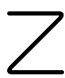
\includegraphics[keepaspectratio]{images/part002_b9f4d066.jpg}}

Remark 2. It follows from Cor. 5 that a maximal torus of G is a maximal commutative subgroup. The converse is not true: for example, in the group \(\mathbf{SO}(3,\mathbf{R})\) , the maximal tori are of dimension 1, and thus cannot contain the subgroup of diagonal matrices, which is isomorphic to \((\mathbf{Z}/2\mathbf{Z})^{2}\) . Moreover, if \(g \in \mathbf{SO}(3,\mathbf{R})\) is a non-scalar diagonal matrix, g is a regular element of \(\mathbf{SO}(3,\mathbf{R})\) whose centralizer is not connected (cf.~Cor. 4).

COROLLARY 6. The maximal tori of G are their own centralizers, and are the fixers of their Lie algebras.

Let T be a maximal torus of G and C its centralizer; since \(L(T)\) is a Cartan subalgebra of \(L(G)\) , we have \(L(T) = L(C)\) , hence C = T since C is connected (Cor. 5).

COROLLARY 7. Let T and T' be two maximal tori of G, A a subset of T and s an automorphism of G that takes A into T'. There exists \(g \in G\) such that \(s \circ (\operatorname{Int} g)\) takes T to T' and coincides with s on A.

Let C be the centralizer of A. Then T and \(s^{-1}(T')\) are two maximal tori of \(C_{0}\) ; every element g of \(C_{0}\) such that \((\operatorname{Int} g)(\mathrm{T}) = s^{-1}(\mathrm{T}')\) has the desired properties.

COROLLARY 8. Let H be a compact Lie group, T a maximal torus of H. Then \(\mathrm{H} = \mathrm{N}_{\mathrm{H}}(\mathrm{T}) \cdot \mathrm{H}_{0}\) , and the injection of \(\mathrm{N}_{\mathrm{H}}(\mathrm{T})\) into H induces an isomorphism from \(\mathrm{N}_{\mathrm{H}}(\mathrm{T}) / \mathrm{N}_{\mathrm{H}_{0}}(\mathrm{T})\) to \(H/H_{0}\) .

Let \(h \in H\) . Then \(h^{-1}Th\) is a maximal torus of \(H_0\) , hence (Th. 2) there exists \(g \in H_0\) such that \(hg \in N_H(T)\) ; thus \(h\) belongs to \(N_H(T).H_0\) , hence the first assertion. The second follows immediately.

Remarks. 3) Let G be a connected Lie group whose Lie algebra is compact. The Cartan subgroups of G are the integral subgroups whose Lie algebras are the Cartan subalgebras of L(G) (the Cartan subgroups of a connected compact group are thus its maximal tori). Theorem 2 and its corollaries remain valid for G, if we replace everywhere the expression ``maximal torus'' by ``Cartan subgroup''. This follows immediately from the fact that, in view of Prop. 5 of §1, no. 4, G is the direct product of a vector group V and a connected compact group K and that the Cartan subgroups of G are the products of V with the maximal tori of K. Moreover, note that it follows from Cor. 6 above that the Cartan subgroups of G can also be defined as the fixers of the Cartan subalgebras of L(G).

* 4) Part \(c\) of Theorem 2 can also be proved in the following way. Give G an invariant riemannian metric (§1, no. 3, Prop. 3). Then, for any element \(g\) of G, there exists a maximal geodesic passing through \(g\) and the identity element of G (Hopf-Rinow theorem), and it can be verified that the closure of such a geodesic is a subtorus of G. *

\subsection{MAXIMAL TORI OF SUBGROUPS AND QUOTIENT GROUPS}

PROPOSITION 1. Let G and G' be two connected compact Lie groups.

\begin{enumerate}
\def\labelenumi{\alph{enumi})}
\item
  Let \(f: \mathbf{G} \to \mathbf{G}'\) be a surjective morphism of Lie groups. The maximal tori of \(\mathbf{G}'\) are the images under \(f\) of the maximal tori of \(\mathbf{G}\) . If the kernel of \(f\) is central in \(\mathbf{G}\) (for example discrete), the maximal tori of \(\mathbf{G}\) are the inverse images under \(f\) of the maximal tori of \(\mathbf{G}'\) .
\item
  Let \(\mathrm{H}\) be a connected closed subgroup of \(\mathrm{G}\) . Every maximal torus of \(\mathrm{H}\) is the intersection with \(\mathrm{H}\) of a maximal torus of \(\mathrm{G}\) .
\item
  Let H be a connected closed normal subgroup of G. The maximal tori of H are the intersections with H of the maximal tori of G.
\item
  Let T be a maximal torus of G; then L(T) is a Cartan subalgebra of L(G) (no. 2, Th. 2 a)), so L(f(T)) is a Cartan subalgebra of L(G') (Chap. VII, §2, no. 1, Cor. 2 of Prop. 4); it follows that f(T) is a maximal torus of G' (no. 2, Th. 2 a)). If Ker f is central in G, it is contained in T (Cor. 2 of Th. 2), so T = \(f^{-1}(f(T))\) .
\end{enumerate}

Conversely, let \(T'\) be a maximal torus of \(G'\) ; we show that there exists a maximal torus T of G such that \(f(\mathrm{T}) = \mathrm{T}'\) . Let \(T_{1}\) be a maximal torus of G; then \(f(\mathrm{T}_{1})\) is a maximal torus of \(G'\) and there exists \(g' \in G'\) such that \(\mathrm{T}' = g' f(\mathrm{T}_{1}) g'^{-1} (\mathrm{Th.~2~b})\) ; if \(g \in G\) is such that \(f(g) = g'\) , we have \(\mathrm{T}' = f(\mathrm{T})\) with \(\mathrm{T} = g\mathrm{T}_{1}g^{-1}\) .

\begin{enumerate}
\def\labelenumi{\alph{enumi})}
\setcounter{enumi}{1}
\item
  Let S be a maximal torus of H; this is a torus of G so there exists a maximal torus T of G containing S. Then \(T \cap H\) is a commutative subgroup of H containing S, hence is equal to S (no. 2, Remark 2).
\item
  By §1, no. 3, Prop. 2 c), L(G) is the direct product of L(H) with an ideal; thus, the Cartan subalgebras of L(H) are the intersections with L(H) of the Cartan subalgebras of L(G). Thus, for any maximal torus T of G, T∩H contains a maximal torus S of H and S = T∩H (no. 2, Remark 2).
\end{enumerate}

Remarks. 1) Proposition 1 generalizes immediately to connected groups with compact Lie algebras. In particular, if G is a connected Lie group whose Lie algebra is compact, the Cartan subgroups of G (cf.~Remark 3, no. 2) are exactly the inverse images of the maximal tori of the connected compact Lie group Ad(G) (under the canonical homomorphism from G to Ad(G)).

\begin{enumerate}
\def\labelenumi{\arabic{enumi})}
\setcounter{enumi}{1}
\tightlist
\item
  Let G be a connected compact Lie group, \(\widetilde{\mathrm{D}}(\mathrm{G})\) the universal covering of the group \(\mathrm{D}(\mathrm{G})\) and \(f : \widetilde{\mathrm{D}}(\mathrm{G}) \to \mathrm{G}\) the composite of the canonical morphisms from \(\tilde{\mathrm{D}}(\mathrm{G})\) to \(\mathrm{D}(\mathrm{G})\) and from \(\mathrm{D}(\mathrm{G})\) to G. Then the map \(T \mapsto f^{-1}(\mathrm{T})\) is a bijection from the set of maximal tori of G to the set of maximal tori of \(\tilde{\mathrm{D}}(\mathrm{G})\) ; the inverse bijection associates to a maximal torus \(\tilde{T}\) of \(\tilde{\mathrm{D}}(\mathrm{G})\) the maximal torus \(\mathrm{C}(\mathrm{G})_{0}.f(\tilde{\mathrm{T}})\) of G.
\end{enumerate}

\subsection{SUBGROUPS OF MAXIMAL RANK}

We shall call the rank of a connected Lie group G the rank of its Lie algebra, and we shall denote it by rk G. By Th. 2 a), the rank of a connected compact Lie group is the common dimension of its maximal tori.

Let G be a connected compact Lie group and H a closed subgroup of G. If H is connected, then \(rkH \leq rkG\) (since the maximal tori of H are tori in G). By Th. 2 c), to say that H is connected and of maximal rank (that is, of rank rkG) means that H is a union of maximal tori of G. We deduce immediately from Proposition 1:

PROPOSITION 2. Let \(f: \mathrm{G} \to \mathrm{G}'\) be a surjective morphism of connected compact Lie groups whose kernel is central. The maps \(\mathrm{H} \mapsto f(\mathrm{H})\) and \(\mathrm{H}' \mapsto f^{-1}(\mathrm{H}')\) are inverse bijections between the set of connected closed subgroups of \(\mathrm{G}\) of maximal rank and the analogous set for \(\mathrm{G}'\) .

PROPOSITION 3. Let G be a connected compact Lie group, and H a connected closed subgroup of maximal rank.

\begin{enumerate}
\def\labelenumi{\alph{enumi})}
\item
  The compact manifold G/H is simply-connected.
\item
  The homomorphism \(\pi_1(\mathrm{H})\to \pi_1(\mathrm{G})\) , induced by the canonical injection of H into G, is surjective.
\end{enumerate}

Since H is connected, we have an exact sequence (General Topology, Chap. XI, in preparation)

\[
\pi_ {1} (\mathrm{H}) \rightarrow \pi_ {1} (\mathrm{G}) \rightarrow \pi_ {1} (\mathrm{G/H}, \bar {e}) \rightarrow 0
\]

where \(\bar{e}\) is the image in G/H of the identity element of G. Since G/H is connected, this immediately implies the equivalence of assertions a) and b). Moreover, if \(f : G' \to G\) is a surjective morphism of connected compact Lie groups whose kernel is central, proving the proposition (in the form a)) for G is the same as proving it for \(G'\) (Prop. 2). Thus, we can first of all replace G by \(\text{Ad}(G)\) , then assume that G is semi-simple, and then by replacing G by a universal covering ( \(\S1\) , no. 4, Cor. 2), assume that G is simply-connected. But then assertion b) is trivial.

PROPOSITION 4. Let G be a compact Lie group, H a connected closed subgroup of G of maximal rank and N the normalizer of H in G. Then H is of finite index in N and is the identity component of N.

Indeed, the Lie algebra of H contains a Cartan subalgebra of L(G). Thus, by Chap. VII, §2, no. 1, Cor. 4 of Prop. 4, H is the identity component of N. Since N is compact, H is of finite index in N.

Remarks. 1) Every integral subgroup H of G such that rkH = rkG is closed: indeed, the preceding proof shows that H is the identity component of its normalizer, which is a closed subgroup of G.

\begin{enumerate}
\def\labelenumi{\arabic{enumi})}
\setcounter{enumi}{1}
\tightlist
\item
  With the notations of Prop. 4, every closed subgroup \(H'\) of G containing H and such that \((H':H)\) is finite normalizes H, and hence is contained in N; similarly, the normalizer of \(H'\) is contained in N. In particular, N is its own normalizer.
\end{enumerate}

\subsection{WEYL GROUP}

Let G be a connected compact Lie group and T a maximal torus of G. Denote by \(N_{G}(T)\) the normalizer of T in G; by Prop. 4 (no. 4), the quotient group \(N_{G}(T)/T\) is finite. We denote it by \(W_{G}(T)\) , or by \(W(T)\) , and call it the Weyl group of the maximal torus T of G, or the Weyl group of G relative to T. Since T is commutative, the operation of \(N_{G}(T)\) on T by inner automorphisms of G induces by passage to the quotient an operation, called the canonical operation, of the group \(W_{G}(T)\) on the Lie group T. By Cor. 6 of Th. 2 of no. 2, this operation is faithful: the associated homomorphism \(W_{G}(T) \rightarrow Aut T\) is injective.

If \(T'\) is another maximal torus of G and if \(g \in G\) is such that Int g maps T to \(T'\) (no. 2, Th. 2 b)), then Int g induces an isomorphism \(a_g\) from \(\mathrm{W}_{\mathrm{G}}(\mathrm{T})\) to \(\mathrm{W}_{\mathrm{G}}(\mathrm{T}')\) and \(a_g(s)(gtg^{-1}) = gs(t)g^{-1}\) for all \(s \in \mathrm{W}_{\mathrm{G}}(\mathrm{T})\) and all \(t \in T\) .

PROPOSITION 5. a) Every conjugacy class of G meets T.

\begin{enumerate}
\def\labelenumi{\alph{enumi})}
\setcounter{enumi}{1}
\tightlist
\item
  The intersections with \(\mathrm{T}\) of the conjugacy classes of \(\mathbf{G}\) are the orbits of the Weyl group.
\end{enumerate}

Let \(g \in \mathbf{G}\) ; by Th. 2 of no. 2, there exists \(h \in \mathbf{G}\) such that \(g \in h\mathrm{Th}^{-1}\) , hence \(a\) ). By definition of the Weyl group, any two elements in the same orbit of \(\mathrm{W_G(T)}\) on \(T\) are conjugate in \(G\) ; conversely, let \(a, b\) be two elements of \(T\) conjugate under \(G\) . There exists \(h \in G\) such that \(b = hah^{-1}\) ; applying Cor. 7 of Th. 2 (no. 2) with \(A = \{a\}\) , \(s = \operatorname{Int} h\) , \(T' = T\) , we see that there exists \(g \in G\) such that \(\operatorname{Int} hg\) maps \(T\) to \(T\) and \(a\) to \(b\) . The class of \(hg\) in \(\mathrm{W_G(T)}\) then maps \(a\) to \(b\) , hence the proposition.

COROLLARY 1. The canonical injection of T into G defines by passage to the quotient a homeomorphism from \(\mathrm{T}/\mathrm{W}_{\mathrm{G}}(\mathrm{T})\) to the space \(\mathrm{G}/\mathrm{Int}(\mathrm{G})\) of conjugacy classes of G.

Indeed, this is a bijective continuous map between two compact spaces (cf.~General Topology, Chap. III, p.~29, Cor. 1).

COROLLARY 2. Let E be a subset of G stable under inner automorphisms. Then E is open (resp. closed, resp. dense) in G if and only if \(E \cap T\) is open (resp. closed, resp. dense) in T.

This follows from Cor. 1 and the fact that the canonical maps \(T \rightarrow T/W_{G}(T)\) and \(G \rightarrow G/Int(G)\) are open (General Topology, Chap. III, p.~10, Lemma 2).

Denote the Lie algebra of G by g, and that of T by t. The operation of \(W_{\mathrm{G}}(\mathrm{T})\) on T induces a representation, called the canonical representation, of the group \(W_{\mathrm{G}}(\mathrm{T})\) on the R-vector space t.

PROPOSITION 6. a) Every orbit of G on g (for the adjoint representation) meets t.

\begin{enumerate}
\def\labelenumi{\alph{enumi})}
\setcounter{enumi}{1}
\tightlist
\item
  The intersections with \(\mathfrak{t}\) of the orbits of \(\mathrm{G}\) are the orbits of \(\mathrm{W_G(T)}\) on \(\mathfrak{t}\) .
\end{enumerate}

Assertion \(a\) ) follows from Th. 1 (no. 1). Let \(x, y\) be two elements of \(\mathfrak{t}\) conjugate under \(\operatorname{Ad}(\mathrm{G})\) , and let \(h \in \mathrm{G}\) be such that \((\operatorname{Ad} h)(x) = y\) . Applying the corollary of Th. 1 (no. 1) with \(\mathfrak{a} = \{x\}\) , \(u = \operatorname{Ad} h, \mathfrak{t}' = \mathfrak{t}\) , we see that there exists \(g \in \mathrm{G}\) such that \(\operatorname{Ad} hg\) maps \(\mathfrak{t}\) to \(\mathfrak{t}\) and \(x\) to \(y\) . Then \(hg \in \mathrm{N}_{\mathrm{G}}(\mathrm{T})\) (Chap. III, §9, no. 4, Prop. 11), and the class of \(hg\) in \(\mathrm{W}_{\mathrm{G}}(\mathrm{T})\) maps \(x\) to \(y\) , hence the proposition.

COROLLARY. The canonical injection of t into g defines by passage to the quotient a homeomorphism from \(\mathfrak{t}/\mathrm{W}_{\mathrm{G}}(\mathrm{T})\) to \(\mathfrak{g}/\mathrm{Ad}(\mathrm{G})\) .

Denote this map by \(j\) ; it is bijective and continuous (Prop. 6). We have a commutative diagram

\[
\begin{array}{c c c} \mathfrak {t} & \stackrel {{i}} {{\longrightarrow}} & \mathfrak {g} \\ p \Big \downarrow & & \Big \downarrow q \\ \mathfrak {t} / \mathrm{W} _ {\mathrm{G}} (\mathrm{T}) & \stackrel {{j}} {{\longrightarrow}} & \mathfrak {g} / \mathrm{Ad} (\mathrm{G}) \end{array}
\]

where p and q are quotient maps, and i is the canonical injection. Since i and q are proper (General Topology, Chap. I, §10, no. 1, Prop. 2 and General Topology, Chap. III, §4, no. 1, Prop. 2 c)) and since p is surjective, it follows that j is proper (General Topology, Chap. I, §10, no. 1, Prop. 5), and hence is a homeomorphism.

PROPOSITION 7. Let H be a closed subgroup of G containing T.

\begin{enumerate}
\def\labelenumi{\alph{enumi})}
\item
  Denote by \(\mathrm{W}_{\mathrm{H}}(\mathrm{T})\) the subgroup \(\mathrm{N}_{\mathrm{H}}(\mathrm{T})/\mathrm{T}\) of \(\mathrm{W}_{\mathrm{G}}(\mathrm{T})\) ; the group \(H/H_{0}\) is isomorphic to the quotient group \(\mathrm{W}_{\mathrm{H}}(\mathrm{T})/\mathrm{W}_{\mathrm{H}_{0}}(\mathrm{T})\) .
\item
  H is connected if and only if every element of \(\mathrm{W}_{\mathrm{G}}(\mathrm{T})\) that has a representative in H belongs to \(\mathrm{W}_{\mathrm{H}_{0}}(\mathrm{T})\) .
\end{enumerate}

Assertion \(a\) ) follows from Cor. 8 of Th. 2 (no. 2), and assertion \(b\) ) is a particular case of \(a\) ).

\subsection{MAXIMAL TORI AND COVERING OF HOMOMORPHISMS}

Let G be a connected compact Lie group, T a maximal torus of G. Consider the derived group \(\mathrm{D}(\mathrm{G})\) of G and its universal covering \(\tilde{\mathrm{D}}(\mathrm{G})\) ; let \(p: \tilde{\mathrm{D}}(\mathrm{G}) \to \mathrm{G}\) be the composite of the canonical morphisms \(\tilde{\mathrm{D}}(\mathrm{G}) \to \mathrm{D}(\mathrm{G})\) and \(\mathrm{D}(\mathrm{G}) \to \mathrm{G}\) . Then \(\tilde{\mathrm{D}}(\mathrm{G})\) is a connected compact Lie group ( \(\S1\) , no. 4, Cor. 2 of Prop. 4); moreover, the inverse image \(\tilde{T}\) of T under p is a maximal torus of \(\tilde{\mathrm{D}}(\mathrm{G})\) (no. 3, Prop. 1).

Lemma 2. Let H be a Lie group, \(f_{\mathrm{T}}: \mathrm{T} \to \mathrm{H}\) and \(\tilde{f}: \tilde{\mathrm{D}}(\mathrm{G}) \to \mathrm{H}\) morphisms of Lie groups such that \(f_{\mathrm{T}}(p(t)) = \tilde{f}(t)\) for all \(t \in \tilde{\mathrm{T}}\) . There exists a unique morphism of Lie groups \(f: \mathrm{G} \to \mathrm{H}\) such that \(f \circ p = \tilde{f}\) and such that the restriction of \(f\) to \(\mathrm{T}\) is \(f_{\mathrm{T}}\) .

Put \(Z = \mathrm{C}(\mathrm{G})_{0}\) ; by §1, no. 4, Cor. 1 of Prop. 4, the morphism of Lie groups \(g: Z \times \tilde{\mathrm{D}}(\mathrm{G}) \to \mathrm{G}\) such that \(g(z, x) = z^{-1} p(x)\) is a covering; its kernel consists of the pairs \((z, x)\) such that \(p(x) = z\) , for which \(x \in p^{-1}(\mathrm{Z}) \subset \tilde{\mathrm{T}}\) . Since the morphism \((z, x) \mapsto f_{\mathrm{T}}(z^{-1}) \tilde{f}(x)\) from \(Z \times \tilde{\mathrm{D}}(\mathrm{G})\) to H maps \(\operatorname{Ker} g\) to \(\{e\}\) , there exists a morphism f from G to H such that \(f \circ p = \tilde{f}\) and \(f(z) = f_{\mathrm{T}}(z)\) for \(z \in Z\) . But we also have \(f(t) = f_{\mathrm{T}}(t)\) for \(t \in p(\tilde{\mathrm{T}})\) ; since \(T = Z.p(\tilde{\mathrm{T}})\) , the restriction of f to T is indeed \(f_{T}\) .

PROPOSITION 8. Let G be a connected compact Lie group, T a maximal torus of G, H a Lie group and \(\varphi : \mathrm{L}(\mathrm{G}) \to \mathrm{L}(\mathrm{H})\) a homomorphism of Lie algebras. There exists a morphism of Lie groups \(f: \mathrm{G} \to \mathrm{H}\) such that \(\mathrm{L}(f) = \varphi\) if and only if there exists a morphism of Lie groups \(f_{\mathrm{T}}: \mathrm{T} \to \mathrm{H}\) such that \(\mathrm{L}(f_{\mathrm{T}}) = \varphi | \mathrm{L}(\mathrm{T})\) ; then \(f_{\mathrm{T}} = f | \mathrm{T}\) .

If \(f: \mathrm{G} \to \mathrm{H}\) is a morphism of Lie groups such that \(\mathrm{L}(f) = \varphi\) , the restriction \(f_{\mathrm{T}}\) of \(f\) to \(\mathrm{T}\) is the unique morphism from \(\mathrm{T}\) to \(\mathrm{H}\) such that \(\mathrm{L}(f_{\mathrm{T}}) = \varphi | \mathrm{L}(\mathrm{T})\) . Conversely, let \(f_{\mathrm{T}}: \mathrm{T} \to \mathrm{H}\) be a morphism of Lie groups such that \(\mathrm{L}(f_{\mathrm{T}}) = \varphi | \mathrm{L}(\mathrm{T})\) . Let \(\tilde{\mathrm{D}}(\mathrm{G})\) and \(p\) be as above; the map \(\mathrm{L}(p)\) induces an isomorphism from \(\mathrm{L}(\tilde{\mathrm{D}}(\mathrm{G}))\) to the derived algebra \(\mathfrak{b}\) of \(\mathrm{L}(\mathrm{G})\) . There exists a morphism of Lie groups \(\tilde{f}: \tilde{\mathrm{D}}(\mathrm{G}) \to \mathrm{H}\) such that \(\mathrm{L}(\tilde{f}) = (\varphi | \mathfrak{b}) \circ \mathrm{L}(p)\) (Chap. III, §6, no. 1, Th. 1). The morphisms \(t \mapsto \tilde{f}(t)\) and \(t \mapsto f_{\mathrm{T}}(p(t))\) from \(\tilde{\mathrm{T}}\) to \(\mathrm{H}\) induce the same homomorphism of Lie algebras, and hence coincide. Applying Lemma 2, we deduce the existence of a morphism \(f: \mathrm{G} \to \mathrm{H}\) such that \(\mathrm{L}(f)\) and \(\varphi\) coincide on \(\mathrm{L}(\mathrm{T})\) and \(\mathfrak{b}\) . Since \(\mathrm{L}(\mathrm{G}) = \mathfrak{b} + \mathrm{L}(\mathrm{T})\) , we have \(\mathrm{L}(f) = \varphi\) .

PROPOSITION 9. Let G be a connected compact Lie group, T a maximal torus of G, H a Lie group and \(f: G \to H\) a morphism. Then f is injective if and only if its restriction to T is injective.

Indeed, by Th. 2 (no. 2) the normal subgroup \(\mathrm{Ker}f\) of G reduces to the identity element if and only if its intersection with T reduces to the identity element.

\section{COMPACT FORMS OF COMPLEX SEMI-SIMPLE LIE ALGEBRAS}

\subsection{REAL FORMS}

If \(\mathfrak{a}\) is a complex Lie algebra, we denote by \(\mathfrak{a}_{[\mathbf{R} ]}\) (or sometimes by \(\mathfrak{a}\) ) the real Lie algebra obtained by restriction of scalars. If \(\mathfrak{g}\) is a real Lie algebra, we denote by \(\mathfrak{g}_{(\mathbf{C})}\) (or sometimes by \(\mathfrak{g}_{\mathbf{C}}\) ) the complex Lie algebra \(\mathbf{C}\otimes_{\mathbf{R}}\mathfrak{g}\) obtained by extension of scalars. The homomorphisms of real Lie algebras \(\mathfrak{g}\to \mathfrak{a}_{[\mathbf{R}]}\) correspond bijectively to the homomorphisms of complex Lie algebras \(\mathfrak{g}_{(\mathbf{C})}\to \mathfrak{a}\) : if \(f:\mathfrak{g}\to \mathfrak{a}_{[\mathbf{R}]}\) and \(g:\mathfrak{g}_{(\mathbf{C})}\to \mathfrak{a}\) correspond, we have \(f(x) = g(1\otimes x)\) and \(g(\lambda \otimes x) = \lambda f(x)\) for \(x\in \mathfrak{g},\lambda \in \mathbf{C}\) .

DEFINITION 1. Let \(\mathfrak{a}\) be a complex Lie algebra. A real form of \(\mathfrak{a}\) is a real subalgebra \(\mathfrak{g}\) of \(\mathfrak{a}\) that is an \(\mathbf{R}\) -structure on the \(\mathbf{C}\) -vector space \(\mathfrak{a}\) (Algebra, Chap. II, §8, no. 1, Def. 1).

This means that the homomorphism of complex Lie algebras \(\mathfrak{g}_{(\mathbf{C})}\to\mathfrak{a}\) associated to the canonical injection \(g\to a_{[R]}\) is bijective. Thus, a real subalgebra g of a is a real form of a if and only if the subspaces g and ig of the real vector space a are complementary. The conjugation of a relative to the real form g is the map \(\sigma:a\to a\) such that

\[
\sigma (x + i y) = x - i y, \quad x, y \in \mathfrak {g}.\tag{1}
\]

PROPOSITION 1. a) Let \(\mathfrak{g}\) be a real form of \(\mathfrak{a}\) and \(\sigma\) the conjugation of \(\mathfrak{a}\) relative to \(\mathfrak{g}\) . Then:

\[
\sigma^ {2} = \mathrm{Id} _ {\mathfrak {a}}, \quad \sigma (\lambda x + \mu y) = \bar {\lambda} \sigma (x) + \bar {\mu} \sigma (y), \quad [ \sigma (x), \sigma (y) ] = \sigma [ x, y ]\tag{2}
\]

for \(\lambda, \mu \in \mathbf{C}\) , \(x, y \in \mathfrak{a}\) . An element \(x\) of \(\mathfrak{a}\) belongs to \(\mathfrak{g}\) if and only if \(\sigma(x) = x\) . b) Let \(\sigma: \mathfrak{a} \to \mathfrak{a}\) be a map satisfying (2). Then the set \(\mathfrak{g}\) of fixed points of \(\sigma\) is a real form of \(\mathfrak{a}\) , and \(\sigma\) is the conjugation of \(\mathfrak{a}\) relative to \(\mathfrak{g}\) .

The proof is immediate.

Note that if B denotes the Killing form of a, and if g is a real form of a, the restriction of B to g is the Killing form of g; in particular, B is real-valued on \(g \times g\) . Assume that a is reductive; then the real Lie algebra g is compact if and only if the restriction of B to g is negative (§1, no. 3). In that case we say that g is a compact real form of a.

\subsection{REAL FORMS ASSOCIATED TO A CHEVALLEY SYSTEM}

In this number, we consider a split semi-simple Lie algebra \((\mathfrak{a},\mathfrak{h})\) over the field \(\mathbf{C}\) (Chap. VIII, §2, no. 1), with root system \(\mathrm{R}(\mathfrak{a},\mathfrak{h}) = \mathrm{R}\) , and a Chevalley system \((X_{\alpha})_{\alpha \in \mathbb{R}}\) of \((\mathfrak{a},\mathfrak{h})\) (Chap. VIII, §2, no. 4, Def. 3).

Recall (loc. cit.) that the linear map \(\theta: a \to a\) that coincides with \(-Id_{h}\) on h and maps \(X_{\alpha}\) to \(X_{-\alpha}\) for all \(\alpha \in R\) is an automorphism of a. Moreover (loc. cit., Prop. 7), if \(\alpha, \beta, \alpha + \beta\) are roots, then

\[
[ X _ {\alpha}, X _ {\beta} ] = \mathrm{N} _ {\alpha , \beta} X _ {\alpha + \beta}\tag{3}
\]

with \(\mathrm{N}_{\alpha ,\beta}\in \mathbf{R}^*\) and

\[
\mathrm{N} _ {- \alpha , - \beta} = \mathrm{N} _ {\alpha , \beta}.\tag{4}
\]

Denote by \(\mathfrak{h}_0\) the real vector subspace of \(\mathfrak{h}\) consisting of the \(H\in \mathfrak{h}\) such that \(\alpha (H)\in \mathbf{R}\) for all \(\alpha \in \mathbb{R}\) . Then \(\mathfrak{h}_0\) is an \(\mathbf{R}\) -structure on the complex vector space \(\mathfrak{h}\) , we have \([X_{\alpha},X_{-\alpha}]\in \mathfrak{h}_0\) for all \(\alpha \in \mathbb{R}\) , and the restriction of the Killing form B of \(\mathfrak{a}\) to \(\mathfrak{h}_0\) is separating positive (Chap. VIII, §2, no. 2, Remark 2). Moreover,

\[
\mathrm{B} (H, X _ {\alpha}) = 0, \quad \mathrm{B} (X _ {\alpha}, X _ {\beta}) = 0 \text {if} \alpha + \beta \neq 0, \quad \mathrm{B} (X _ {\alpha}, X _ {- \alpha}) <   0\tag{5}
\]

(Chap. VIII, §2, no. 2, Prop. 1 and no. 4, Lemma 3).

PROPOSITION 2. a) The real vector subspace \(\mathfrak{a}_0 = \mathfrak{h}_0 + \sum_{\alpha \in \mathrm{R}} \mathbf{R}X_\alpha\) of \(\mathfrak{a}\) is a real form of \(\mathfrak{a}\) , of which \(\mathfrak{h}_0\) is a Cartan subalgebra. The pair \((\mathfrak{a}_0, \mathfrak{h}_0)\) is a split semi-simple real Lie algebra, of which \((X_\alpha)\) is a Chevalley system.

\begin{enumerate}
\def\labelenumi{\alph{enumi})}
\setcounter{enumi}{1}
\tightlist
\item
  Let \(\sigma\) be the conjugation of \(\mathfrak{a}\) relative to \(\mathfrak{a}_0\) . Then \(\sigma \circ \theta = \theta \circ \sigma\) . The set of fixed points of \(\sigma \circ \theta\) is a compact real form \(\mathfrak{a}_u\) of \(\mathfrak{a}\) , of which \(i\mathfrak{h}_0\) is a Cartan subalgebra.
\end{enumerate}

Part a) follows immediately from the preceding. We prove b). Since \(\sigma\circ\theta\) and \(\theta\circ\sigma\) are two semi-linear maps from a to a that coincide on \(a_{0}\) , they coincide. Now \(\sigma\circ\theta\) satisfies conditions (2) of no. 1, hence is the conjugation of a relative to the real form \(a_{u}\) consisting of the \(x\in a\) such that \(\sigma\circ\theta(x)=x\) (Prop. 1). For all \(\alpha\in R\) put

\[
u _ {\alpha} = X _ {\alpha} + X _ {- \alpha}, v _ {\alpha} = i (X _ {\alpha} - X _ {- \alpha}).\tag{6}
\]

Then the R-vector space \(a_{u}\) is generated by \(ih_{0}\) , the \(u_{\alpha}\) and the \(v_{\alpha}\) . More precisely, if we choose a chamber C of R, then

\[
\mathfrak {a} _ {u} = i \mathfrak {h} _ {0} \oplus \bigoplus_ {\alpha \in \mathrm{R} _ {+} (\mathrm{C})} \left(\mathbf {R} u _ {\alpha} + \mathbf {R} v _ {\alpha}\right).\tag{7}
\]

It is clear that \(i\mathfrak{h}_0\) is a Cartan subalgebra of \(\mathfrak{a}_u\) , and it remains to prove that the restriction of \(B\) to \(\mathfrak{a}_u\) is negative. Now \(i\mathfrak{h}_0\) and the different subspaces of the form \(\mathbf{R}u_{\alpha}\oplus \mathbf{R}v_{\alpha}\) are orthogonal with respect to B, by (5); the restriction of B to \(i\mathfrak{h}_0\) is negative and

\[
\mathrm{B} (u _ {\alpha}, u _ {\alpha}) = \mathrm{B} (v _ {\alpha}, v _ {\alpha}) = 2 \mathrm{B} (X _ {\alpha}, X _ {- \alpha}) <   0, \quad \mathrm{B} (u _ {\alpha}, v _ {\alpha}) = 0,\tag{8}
\]

hence the conclusion.

Remark. With the preceding notations, we have the following formulas:

\[
[ h, u _ {\alpha} ] = - i \alpha (h) v _ {\alpha}, [ h, v _ {\alpha} ] = i \alpha (h) u _ {\alpha}, [ u _ {\alpha}, v _ {\alpha} ] = 2 i H _ {\alpha}, (h \in \mathfrak {h})\tag{9}
\]

\[
[ u _ {\alpha}, u _ {\beta} ] = \mathrm{N} _ {\alpha , \beta} u _ {\alpha + \beta} + \mathrm{N} _ {\alpha , - \beta} u _ {\alpha - \beta}, \quad \alpha \neq \pm \beta ,\tag{10}
\]

\[
[ v _ {\alpha}, v _ {\beta} ] = - \mathrm{N} _ {\alpha , \beta} u _ {\alpha + \beta} + \mathrm{N} _ {\alpha , - \beta} u _ {\alpha - \beta}, \quad \alpha \neq \pm \beta ,\tag{11}
\]

\[
[ u _ {\alpha}, v _ {\beta} ] = \mathrm{N} _ {\alpha , \beta} v _ {\alpha + \beta} - \mathrm{N} _ {\alpha , - \beta} v _ {\alpha - \beta}, \quad \alpha \neq \pm \beta ,\tag{12}
\]

(in the last three formulas, it is understood, as usual, that \(\mathrm{N}_{\gamma, \delta} = 0\) if \(\gamma + \delta\) is not a root).

Note that \(\sum \mathbf{R}u_{\alpha}\) is a real subalgebra of \(\mathfrak{a}\) , namely \(\mathfrak{a}_0 \cap \mathfrak{a}_u\) .

Let \(\mathrm{Q}(\mathrm{R})\) be the group of radical weights of R (Chap. VI, §1, no. 9). Recall that to any homomorphism \(\gamma : \mathrm{Q}(\mathrm{R}) \to \mathbf{C}^*\) is associated an elementary automorphism \(f(\gamma)\) of \(\mathfrak{a}\) such that \(f(\gamma)(h) = h\) for all \(h \in \mathfrak{h}\) and \(f(\gamma)X_{\alpha} = \gamma(\alpha)X_{\alpha}\) (Chap. VIII, §5, no. 2).

PROPOSITION 3. Let \(\mathfrak{g}\) be a compact real form of \(\mathfrak{a}\) such that \(\mathfrak{g} \cap \mathfrak{h} = i\mathfrak{h}_0\) . There exists a homomorphism \(\gamma: \mathrm{Q}(\mathrm{R}) \to \mathbf{R}_{+}^{*}\) such that \(\mathfrak{g} = f(\gamma)(\mathfrak{a}_u)\) .

Let \(\tau\) be the conjugation of \(\mathfrak{a}\) relative to \(\mathfrak{g}\) . By hypothesis \(\tau(x) = x\) for \(x \in i\mathfrak{h}_0\) , so \(\tau(x) = -x\) for \(x \in \mathfrak{h}_0\) . Thus, for all \(\alpha \in \mathrm{R}\) and all \(h \in \mathfrak{h}_0\) ,

\[
[ h, \tau (X _ {\alpha}) ] = [ - \tau (h), \tau (X _ {\alpha}) ] = - \tau ([ h, X _ {\alpha} ]) = - \tau (\alpha (h) X _ {\alpha});
\]

it follows that \([h, \tau(X_{\alpha})] = -\alpha(h)\tau(X_{\alpha})\) for all \(h \in \mathfrak{h}_0\) , hence also for all \(h \in \mathfrak{h}\) . Hence there exists \(c_{\alpha} \in \mathbf{C}^*\) such that \(\tau(X_{\alpha}) = c_{\alpha}X_{-\alpha}\) . Since \([X_{\alpha}, X_{-\alpha}] \in \mathfrak{h}_0\) , we have \([\tau(X_{\alpha}), \tau(X_{-\alpha})] = -[X_{\alpha}, X_{-\alpha}]\) , so \(c_{\alpha}c_{-\alpha} = 1\) ; similarly, formulas (3) and (4) give \(c_{\alpha + \beta} = c_{\alpha}c_{\beta}\) if \(\alpha, \beta, \alpha + \beta\) are roots. By Chap. VI, §1, no. 6, Cor. 2 of Prop. 19, there exists a homomorphism \(\delta: \mathrm{Q}(\mathrm{R}) \to \mathbf{C}^*\) such that \(\delta(\alpha) = c_{\alpha}\) for all \(\alpha \in \mathrm{R}\) .

We now show that each \(c_{\alpha}\) is strictly positive. Indeed, \(c_{\alpha}\mathrm{B}(X_{\alpha},X_{-\alpha})=\mathrm{B}(X_{\alpha},\tau(X_{\alpha}))\) , and since \(\mathrm{B}(X_{\alpha},X_{-\alpha})\) is negative, it suffices to show that \(\mathrm{B}(z,\tau(z))<0\) for every non-zero element z of a; but every element of a can be written as \(x+iy\) , with x and y in g, and

\[
\mathrm{B} (x + i y, \tau (x + i y)) = \mathrm{B} (x + i y, x - i y) = \mathrm{B} (x, x) + \mathrm{B} (y, y),
\]

hence the stated assertion, the restriction of B to g being negative and separating by hypothesis.

It follows that the homomorphism \(\delta\) takes values in \(\mathbf{R}_+^*\) ; hence there exists a homomorphism \(\gamma : \mathrm{Q}(\mathrm{R}) \to \mathbf{R}_+^*\) such that \(\delta = \gamma^{-2}\) . Then \(f(\gamma)^{-1}(\mathfrak{g})\) is a real form of \(\mathfrak{a}\) ; the corresponding conjugation is \(\tau' = f(\gamma)^{-1} \circ \tau \circ f(\gamma)\) . For all \(\alpha \in \mathbb{R}\) , we have

\[
\tau^ {\prime} (X _ {\alpha}) = f (\gamma) ^ {- 1} (\tau (c _ {\alpha} ^ {- 1 / 2} X _ {\alpha})) = f (\gamma) ^ {- 1} (c _ {\alpha} ^ {1 / 2} X _ {- \alpha}) = X _ {- \alpha},
\]

and \(\tau'(h) = \tau(h) = h\) for \(h \in i\mathfrak{h}_0\) ; it follows that \(\tau'\) is the conjugation with respect to \(\mathfrak{a}_u\) , and hence that \(f(\gamma)^{-1}(\mathfrak{g}) = \mathfrak{a}_u\) .

\subsection{CONJUGACY OF COMPACT FORMS}

THEOREM 1. Let \(\mathfrak{a}\) be a complex semi-simple Lie algebra.

\begin{enumerate}
\def\labelenumi{\alph{enumi})}
\item
  \(\mathfrak{a}\) has compact (resp. splittable) real forms.
\item
  The group \(\operatorname{Int}(\mathfrak{a})\) operates transitively on the set of compact (resp. splittable) real forms of a.
\end{enumerate}

Let \(\mathfrak{h}\) be a Cartan subalgebra of \(\mathfrak{a}\) . Then \((\mathfrak{a},\mathfrak{h})\) is split (Chap. VIII, §2, no. 1, Remark 2), and has a Chevalley system \((X_{\alpha})\) (Chap. VIII, §4, no. 4, Cor. of Prop. 5). Part \(a)\) now follows from Prop. 2. Let \(\mathfrak{g}\) be a compact real form of \(\mathfrak{a}\) ; we show that there exists \(v\in\mathrm{Int}(\mathfrak{a})\) such that \(v(\mathfrak{a}_{u})=\mathfrak{g}\) . Let \(\mathfrak{t}\) be a Cartan subalgebra of \(\mathfrak{g}\) ; then \(\mathfrak{t}_{(\mathbf{C})}\) is a Cartan subalgebra of \(\mathfrak{a}\) ; since \(\mathrm{Int}(\mathfrak{a})\) operates transitively on the set of Cartan subalgebras of \(\mathfrak{a}\) (Chap. VII, §3, no. 2, Th. 1), we are reduced to the case in which \(\mathfrak{t}_{(\mathbf{C})}=\mathfrak{h}\) . Since \(\mathfrak{g}\) is a compact form, the eigenvalues of the endomorphisms ad \(h\) , for \(h\in\mathfrak{t}\) , are purely imaginary ( \(\S1\) , no. 3, Prop. 1), so the roots \(\alpha\in\mathbb{R}\) map \(\mathfrak{t}\) to \(i\mathbf{R}\) ; this implies that \(\mathfrak{t}=i\mathfrak{h}_{0}\) . Then, by Prop. 3 (no. 2), there exists \(v\in\mathrm{Int}(\mathfrak{a})\) such that \(v(\mathfrak{a}_{u})=\mathfrak{g}\) , hence \(b)\) in the case of compact forms. Finally, let \(\mathfrak{m}_{1}\) and \(\mathfrak{m}_{2}\) be two splittable real forms of \(\mathfrak{a}\) . There exist framings \((\mathfrak{m}_{1},\mathfrak{h}_{1},\mathrm{B}_{1},(X_{\alpha}^{1}))\) and \((\mathfrak{m}_{2},\mathfrak{h}_{2},\mathrm{B}_{2},(X_{\alpha}^{2}))\) (Chap. VIII, §4, no. 1). These extend in an obvious way to bases \(e_{1}\) and \(e_{2}\) of \(\mathfrak{a}\) . An automorphism of \(\mathfrak{a}\) that maps \(e_{1}\) to \(e_{2}\) maps \(\mathfrak{m}_{1}\) to \(\mathfrak{m}_{2}\) ; thus, it suffices to apply Prop. 5 of Chap. VIII, §5, no. 3, to obtain the existence of an element \(u\) of \(\mathrm{Aut}_{0}(\mathfrak{a})=\mathrm{Int}(\mathfrak{a})\) such that \(u(\mathfrak{m}_{1})=\mathfrak{m}_{2}\) .

Remark. We shall see much later a general classification of real forms of a complex semi-simple Lie algebra.

COROLLARY 1. Let \(\mathfrak{g}\) and \(\mathfrak{g}'\) be two compact real Lie algebras. Then \(\mathfrak{g}\) and \(\mathfrak{g}'\) are isomorphic if and only if the complex Lie algebras \(\mathfrak{g}_{(\mathbf{C})}\) and \(\mathfrak{g}'_{(\mathbf{C})}\) are isomorphic.

The condition is clearly necessary. Conversely, assume that \(\mathfrak{g}_{(\mathbf{C})}\) and \(\mathfrak{g}'_{(\mathbf{C})}\) are isomorphic. Let c (resp. \(c'\) ) be the centre of g (resp. \(g'\) ) and s (resp. \(s'\) ) the derived algebra of g (resp. \(g'\) ). Then \(\mathfrak{c}_{(\mathbf{C})}\) and \(\mathfrak{c}'_{(\mathbf{C})}\) are the centres of \(\mathfrak{g}_{(\mathbf{C})}\) and \(\mathfrak{g}'_{(\mathbf{C})}\) , respectively, and hence are isomorphic; it follows that the commutative algebras c and \(c'\) are isomorphic. Similarly, \(\mathfrak{s}_{(\mathbf{C})}\) and \(\mathfrak{s}'_{(\mathbf{C})}\) are isomorphic, hence s and \(s'\) , which are compact real forms of two isomorphic complex semi-simple Lie algebras, are isomorphic by Th. 1 b).

COROLLARY 2. Let \(\mathfrak{a}\) be a complex Lie algebra. The following conditions are equivalent:

\begin{enumerate}
\def\labelenumi{(\roman{enumi})}
\item
  \(\mathfrak{a}\) is reductive.
\item
  There exists a compact real Lie algebra \(\mathfrak{g}\) such that \(\mathfrak{a}\) is isomorphic to \(\mathfrak{g}(\mathbf{C})\) .
\item
  There exists a compact Lie group \(\mathbf{G}\) such that \(\mathfrak{a}\) is isomorphic to \(\mathrm{L}(\mathrm{G})_{(\mathbf{C})}\) .
\end{enumerate}

By Def. 1 of §1, no. 3, conditions (ii) and (iii) are equivalent and imply (i). If \(\mathfrak{a}\) is reductive, it is the direct product of a commutative algebra, which clearly has a compact real form, and a semi-simple algebra which has one by Th. 1 \(a\) ), hence (i) implies (ii).

COROLLARY 3. Let \(\mathfrak{a}_1\) and \(\mathfrak{a}_2\) be two complex semi-simple Lie algebras. The compact real forms of \(\mathfrak{a}_1 \times \mathfrak{a}_2\) are the products \(\mathfrak{g}_1 \times \mathfrak{g}_2\) , where, for \(i = 1, 2\) , \(\mathfrak{g}_i\) is a compact real form of \(\mathfrak{a}_i\) .

Indeed, there exists a compact real form \(g_{1}\) (resp. \(g_{2}\) ) of \(a_{1}\) (resp. \(a_{2}\) ); then \(g_{1} \times g_{2}\) is a compact real form of \(a_{1} \times a_{2}\) . The corollary now follows from Th. 1 b), applied to \(a_{1}, a_{2}\) and \(a_{1} \times a_{2}\) .

Note that it follows from Cor. 3 above that a compact real Lie algebra g is simple if and only if the complex Lie algebra \(\mathfrak{g}_{(\mathbf{C})}\) is simple. We say that g is of type \(A_{n}\) , or \(B_{n}, \ldots\) , if \(\mathfrak{g}_{(\mathbf{C})}\) is of type \(A_{n}\) , or \(B_{n}, \ldots\) (Chap. VIII, §2, no. 2). By Cor. 1 above, two compact simple real Lie algebras are isomorphic if and only if they are of the same type.

Let G be an almost simple connected compact Lie group (Chap. III, §9, no. 8, Def. 3). We say that G is of type \(A_{n}\) , or \(B_{n}\) , \ldots, if its Lie algebra is of type \(A_{n}\) , or \(B_{n}\) , \ldots. Two simply-connected almost simple compact Lie groups are isomorphic if and only if they are of the same type.

\subsection{\texorpdfstring{EXAMPLE I: COMPACT ALGEBRAS OF TYPE \(A_{n}\)}{EXAMPLE I: COMPACT ALGEBRAS OF TYPE A\_\{n\}}}

Let V be a finite dimensional complex vector space and \(\Phi\) a separating positive hermitian form on V. The unitary group associated to \(\Phi\) (cf.~Algebra, Chap. IX) is the subgroup \(\mathbf{U}(\Phi)\) of \(\mathbf{GL}(V)\) consisting of the automorphisms of the complex Hilbert space \((V,\Phi)\) ; this is a (real) Lie subgroup of the group \(\mathbf{GL}(V)\) , whose Lie algebra is the subalgebra \(\mathfrak{u}(\Phi)\) of the real Lie algebra \(\mathfrak{gl}(V)\) consisting of the endomorphisms x of V such that \(x^{*} = -x\) (Chap. III, §3, no. 10, Cor. 2 of Prop. 37), where \(x^{*}\) denotes the adjoint of x relative to \(\Phi\) . Since the group \(\mathbf{U}(\Phi)\) is compact (§1, no. 1), \(\mathfrak{u}(\Phi)\) is a compact real Lie algebra. Similarly, the special unitary group \(\mathbf{SU}(\Phi) = \mathbf{U}(\Phi) \cap \mathbf{SL}(V)\) is a compact Lie subgroup of \(\mathbf{SL}(V)\) , whose Lie algebra is \(\mathfrak{su}(\Phi) = \mathfrak{u}(\Phi) \cap \mathfrak{sl}(V)\) .

When \(V = C^{n}\) and \(\varPhi\) is the usual hermitian form (for which the canonical basis of \(C^{n}\) is orthonormal), we write \(\mathbf{U}(n, \mathbf{C})\) , \(\mathbf{SU}(n, \mathbf{C})\) , \(\mathfrak{u}(n, \mathbf{C})\) , \(\mathfrak{s}\mathfrak{u}(n, \mathbf{C})\) instead of \(\mathbf{U}(\varPhi)\) , \(\mathbf{SU}(\varPhi)\) , \(\mathfrak{u}(\varPhi)\) , \(\mathfrak{s}\mathfrak{u}(\varPhi)\) . The elements of \(\mathbf{U}(n, \mathbf{C})\) (resp. \(\mathfrak{u}(n, \mathbf{C})\) )

are the matrices \(A \in \mathrm{M}_{n}(\mathbf{C})\) such that \(A.^{t}\bar{A} = I_{n}\) (resp. \(A = -^{t}\bar{A}\) ), which are said to be unitary (resp. anti-hermitian).

PROPOSITION 4. a) The compact real forms of the complex Lie algebra \(\mathfrak{sl}(V)\) are the algebras \(\mathfrak{su}(\Phi)\) , where \(\Phi\) belongs to the set of separating positive hermitian forms on the complex vector space \(V\) .

\begin{enumerate}
\def\labelenumi{\alph{enumi})}
\setcounter{enumi}{1}
\tightlist
\item
  The algebras \(\mathfrak{u}(\varPhi)\) are the compact real forms of \(\mathfrak{gl}(\mathrm{V})\) .
\end{enumerate}

Let \(\varPhi\) be a separating positive hermitian form on V. For all \(x\in\mathfrak{gl}(V)\) , put \(\sigma(x)=-x^{*}\) (where \(x^{*}\) is the adjoint of \(x\) relative to \(\varPhi\) ). Then \(\sigma\) satisfies conditions (2) of Prop. 1 of no. 1, so the set \(\mathfrak{u}(\varPhi)\) (resp. \(\mathfrak{su}(\varPhi)\) ) of fixed points of \(\sigma\) on \(\mathfrak{gl}(V)\) (resp. \(\mathfrak{sl}(V)\) ) is a compact real form of \(\mathfrak{gl}(V)\) (resp. \(\mathfrak{sl}(V)\) ). Since \(\mathbf{GL}(V)\) operates transitively on the set of separating positive hermitian forms on V (Algebra, Chap. IX) and on the set of compact real forms of \(\mathfrak{sl}(V)\) (no. 3, Th. 1 and Chap. VIII, §13, no. 1 (VII)), Prop. 4 is proved.

COROLLARY. Every compact simple real Lie algebra of type \(\mathrm{A}_n\) ( \(n \geq 1\) ) is isomorphic to \(\mathfrak{su}(n + 1, \mathbf{C})\) .

Indeed, every complex Lie algebra of type \(\mathbf{A}_n\) is isomorphic to \(\mathfrak{sl}(n + 1,\mathbf{C})\) (Chap. VIII, §13, no. 1).

Remarks. 1) We have \(\mathfrak{gl}(\mathrm{V}) = \mathfrak{sl}(\mathrm{V}) \times \mathbf{C}.1_{\mathrm{V}}\) , \(\mathfrak{u}(\varPhi) = \mathfrak{su}(\varPhi) \times \mathbf{R}.i1_{\mathrm{V}}\) ; the compact real forms of \(\mathfrak{gl}(\mathrm{V})\) are the \(\mathfrak{su}(\varPhi) \times \mathbf{R}. \alpha 1_{\mathrm{V}}, \alpha \in \mathbf{C}^*\) .

\begin{enumerate}
\def\labelenumi{\arabic{enumi})}
\setcounter{enumi}{1}
\tightlist
\item
  If the complex Lie algebra \(\mathfrak{a} = \mathfrak{sl}(n,\mathbf{C})\) is equipped with the splitting and Chevalley system introduced in Chap. VIII, §13, no. 1 (IX), then, with the notations in no. 2,
\end{enumerate}

\[
\mathfrak {a} _ {u} = \mathfrak {s u} (n, \mathbf {C}), \quad \mathfrak {a} _ {0} = \mathfrak {s l} (n, \mathbf {R}), \quad \mathfrak {a} _ {u} \cap \mathfrak {a} _ {0} = \mathfrak {o} (n, \mathbf {R}).
\]

\subsection{\texorpdfstring{EXAMPLE II: COMPACT ALGEBRAS OF TYPE \(\mathbf{B}_n\) AND \(\mathbf{D}_n\)}{EXAMPLE II: COMPACT ALGEBRAS OF TYPE \textbackslash mathbf\{B\}\_n AND \textbackslash mathbf\{D\}\_n}}

Let V be a finite dimensional real vector space and Q a separating positive quadratic form on V. The orthogonal group associated to Q (Algebra, Chap. IX) is the subgroup \(\mathbf{O}(\mathbf{Q})\) of \(\mathbf{GL}(\mathbf{V})\) consisting of the automorphisms of the real Hilbert space (V, Q); this is a Lie subgroup of \(\mathbf{GL}(\mathbf{V})\) , whose Lie algebra is the subalgebra \(\mathfrak{o}(\mathbf{Q})\) of \(\mathfrak{gl}(\mathbf{V})\) consisting of the endomorphisms x of V such that \(x^{*} = -x\) (Chap. III, §3, no. 10, Cor. 2 of Prop. 37), \(x^{*}\) denoting the adjoint of x relative to Q. Since the group \(\mathbf{O}(\mathbf{Q})\) is compact, \(\mathfrak{o}(\mathbf{Q})\) is thus a compact real Lie algebra. Put \(\mathbf{SO}(\mathbf{Q}) = \mathbf{O}(\mathbf{Q}) \cap \mathbf{SL}(\mathbf{V})\) ; this is a closed subgroup of finite index of \(\mathbf{O}(\mathbf{Q})\) (of index 2 if dim V ≠ 0), hence also with Lie algebra \(\mathfrak{o}(\mathbf{Q})\) .

When \(V = R^{n}\) and Q is the usual quadratic form (for which the canonical basis of \(R^{n}\) is orthonormal), we write \(\mathbf{O}(n, \mathbf{R})\) , \(\mathbf{SO}(n, \mathbf{R})\) , \(\mathfrak{o}(n, \mathbf{R})\) instead of \(\mathbf{O}(\mathbf{Q})\) , \(\mathbf{SO}(\mathbf{Q})\) , \(\mathfrak{o}(\mathbf{Q})\) . The elements of \(\mathbf{O}(n, \mathbf{R})\) (resp. \(\mathfrak{o}(n, \mathbf{R})\) ) are the matrices

\(A \in \mathrm{M}_n(\mathbf{R})\) such that \(A.^t A = I_n\) (resp. \(A = -^t A\) ), which are said to be orthogonal (resp. anti-symmetric).

Let \(\mathrm{V}_{(\mathbf{C})}\) be the complex vector space associated to \(\mathrm{V}\) and let \(\mathrm{Q}_{(\mathbf{C})}\) be the quadratic form on \(\mathrm{V}_{(\mathbf{C})}\) associated to \(\mathbf{Q}\) . Identify \(\mathfrak{gl}(\mathrm{V})_{(\mathbf{C})}\) with \(\mathfrak{gl}(\mathrm{V}_{(\mathbf{C})})\) ; then \(\mathfrak{o}(\mathrm{Q})_{(\mathbf{C})}\) is identified with \(\mathfrak{o}(\mathrm{Q}_{(\mathbf{C})})\) : this is clear since the map \(x \mapsto x^{*} + x\) from \(\mathfrak{gl}(\mathrm{V}_{(\mathbf{C})})\) to itself is \(\mathbf{C}\) -linear. Since \(\mathfrak{o}(\mathrm{Q}_{(\mathbf{C})})\) is of type \(\mathrm{B}_n\) if \(\dim V = 2n + 1\) , \(n \geq 1\) , and of type \(\mathrm{D}_n\) if \(\dim V = 2n\) , \(n \geq 3\) (Chap. VIII, §13, nos. 2 and 4), we deduce:

PROPOSITION 5. Every compact simple real Lie algebra of type \(B_{n}\) , \(n \geq 1\) (resp. of type \(D_{n}\) , \(n \geq 3\) ) is isomorphic to \(\mathfrak{o}(2n + 1, \mathbf{R})\) (resp. \(\mathfrak{o}(2n, \mathbf{R})\) ).

\subsection{COMPACT GROUPS OF RANK 1}

By General Topology, Chap. VIII, §1, no. 4, Prop. 3, Prop. 4 and Remark 4, the topological group \(\mathbf{SU}(2,\mathbf{C})\) is isomorphic to the topological group \(\mathbf{S}_3\) of quaternions of norm 1, and the quotient of \(\mathbf{SU}(2,\mathbf{C})\) by the subgroup Z consisting of the matrices \(I_2\) and \(-I_2\) is isomorphic to the topological group \(\mathbf{SO}(3,\mathbf{R})\) . Note that Z is the centre of \(\mathbf{SU}(2,\mathbf{C})\) : indeed, since \(\mathbf{H} = \mathbf{R}.\mathbf{S}_3\) , every element of the centre of the group \(\mathbf{S}_3\) is in the centre \(\mathbf{R}\) of the algebra \(\mathbf{H}\) and hence belongs to the group with two elements \(\mathbf{S}_3 \cap \mathbf{R} = \{-1,1\}\) .

PROPOSITION 6. Every compact semi-simple real Lie algebra of rank 1 is isomorphic to \(\mathfrak{su}(2,\mathbf{C})\) and to \(\mathfrak{o}(3,\mathbf{R})\) . Every connected semi-simple compact Lie group of rank 1 is isomorphic to \(\mathbf{SU}(2,\mathbf{C})\) if it is simply-connected, and to \(\mathbf{SO}(3,\mathbf{R})\) if not.

The first assertion follows from the Cor. of Prop. 4 and Prop. 5. Since \(\mathbf{SU}(2,\mathbf{C})\) is homeomorphic to \(\mathbf{S}_3\) (General Topology, Chap. VIII, §1, no. 4, Remark 4), hence is simply-connected (General Topology, Chap. XI, in preparation), every simply-connected compact semi-simple Lie group of rank 1 is isomorphic to \(\mathbf{SU}(2,\mathbf{C})\) ; every connected compact semi-simple Lie group of rank 1 that is not simply-connected is isomorphic to a quotient of \(\mathbf{SU}(2,\mathbf{C})\) by a subgroup of \(Z\) that does not reduce to the identity element, hence to \(\mathbf{SO}(3,\mathbf{R})\) .

Remark. We have seen above that \(\mathbf{SU}(2,\mathbf{C})\) is simply-connected and that \(\pi_{1}(\mathbf{SO}(3,\mathbf{R}))\) is of order 2. We shall see much later that these results generalize to \(\mathbf{SU}(n,\mathbf{C})\) ( \(n\geq1\) ) and \(\mathbf{SO}(n,\mathbf{R})\) ( \(n\geq3\) ), respectively (cf.~also §3, Exerc. 4 and 5).

Recall (Chap. VIII, §1, no. 1) that the canonical basis of \(\mathfrak{sl}(2,\mathbf{C})\) is the basis \((X_{+},X_{-},H)\) , where

\[
X _ {+} = \left( \begin{array}{c c} 0 & 1 \\ 0 & 0 \end{array} \right), X _ {-} = \left( \begin{array}{c c} 0 & 0 \\ - 1 & 0 \end{array} \right), H = \left( \begin{array}{c c} 1 & 0 \\ 0 & - 1 \end{array} \right).
\]

We thus obtain a basis \((U, V, iH)\) of \(\mathfrak{su}(2, \mathbf{C})\) , also called canonical, by putting

\[
\begin{array}{c} U = X _ {+} + X _ {-} = \left( \begin{array}{c c} 0 & 1 \\ - 1 & 0 \end{array} \right), V = i (X _ {+} - X _ {-}) = \left( \begin{array}{c c} 0 & i \\ i & 0 \end{array} \right), \\ i H = \left( \begin{array}{c c} i & 0 \\ 0 & - i \end{array} \right). \end{array}
\]

We have

\[
[ i H, U ] = 2 V, [ i H, V ] = - 2 U, [ U, V ] = 2 i H.\tag{13}
\]

If B denotes the Killing form of \(\mathfrak{su}(2,\mathbf{C})\) an immediate calculation gives

\[
\mathrm{B} (a U + b V + c i H, a ^ {\prime} U + b ^ {\prime} V + c ^ {\prime} i H) = - 8 (a a ^ {\prime} + b b ^ {\prime} + c c ^ {\prime}),\tag{14}
\]

so that, if we identify \(\mathfrak{su}(2,\mathbf{C})\) with \(R^{3}\) by means of the canonical basis, the adjoint representation of \(\mathbf{SU}(2,\mathbf{C})\) defines a homomorphism \(\mathbf{SU}(2,\mathbf{C})\to\mathbf{SO}(3,\mathbf{R})\) (cf.~above).

Further, note that \(\mathbf{Ri}H\) is a Cartan subalgebra of \(\mathfrak{su}(2,\mathbf{C})\) , that the maximal torus \(T\) of \(\mathbf{SU}(2,\mathbf{C})\) that corresponds to it consists of the diagonal matrices \(\left( \begin{array}{cc}a & 0\\ 0 & \bar{a} \end{array} \right)\) , where \(a\bar{a} = 1\) , and that the exponential map

\(\exp : \mathbf{R}iH \to \mathrm{T}\)

maps \(xH\) , for \(x \in \mathbf{R}i\) , to the matrix \(\left( \begin{array}{cc}\exp (x) & 0\\ 0 & \exp (-x) \end{array} \right)\) , and thus has kernel \(\mathbf{Z}.K\) , where \(K\) is the element of \(\mathfrak{su}(2,\mathbf{C})\) defined by

\[
K = 2 \pi i H = \left( \begin{array}{c c} 2 \pi i & 0 \\ 0 & - 2 \pi i \end{array} \right).\tag{15}
\]

Further, the centre of \(\mathbf{SU}(2,\mathbf{C})\) consists of the identity and \(\exp (K / 2)\) .

\[
\theta = \left( \begin{array}{c c} 0 & - 1 \\ 1 & 0 \end{array} \right) \in \mathbf {S U} (2, \mathbf {C}).\tag{16}
\]

By Chap. VIII, §1, no. 5,

\[
\theta^ {2} = \left( \begin{array}{c c} - 1 & 0 \\ 0 & - 1 \end{array} \right), (\text {Int}   \theta) t = t ^ {- 1}, t \in \text {T},\tag{17}
\]

\[
(\operatorname{Ad} \theta) X _ {+} = X _ {-}, (\operatorname{Ad} \theta) X _ {-} = X _ {+}, (\operatorname{Ad} \theta) U = U, (\operatorname{Ad} \theta) V = - V.\tag{18}
\]

\[
\text {   Finally,   for   } t = \left( \begin{array}{c c} a & 0 \\ 0 & \bar {a} \end{array} \right) \in \mathrm{T}, \text {   we   have   }
\]

\[
(\operatorname{Ad} t) X _ {+} = a ^ {2} X _ {+}, (\operatorname{Ad} t) X _ {-} = a ^ {- 2} X _ {-}, (\operatorname{Ad} t) H = H,\tag{19}
\]

\[
(\operatorname{Ad} t) U = \mathcal {R} (a ^ {2}) U + \mathcal {I} (a ^ {2}) V, (\operatorname{Ad} t) V = - \mathcal {I} (a ^ {2}) U + \mathcal {R} (a ^ {2}) V.\tag{20}
\]

\section{ROOT SYSTEM ASSOCIATED TO A COMPACT GROUP}

In paragraphs 4 to 8, we denote by G a connected compact Lie group and by T a maximal torus of G. We denote by g (resp. t) the Lie algebra of G (resp. T), by gC (resp. tC) the complexified Lie algebra of g (resp. t), and by W the Weyl group of G relative to T (§2, no. 5).

\subsection{THE GROUP X(H)}

Let H be a compact Lie group. Denote by X(H) the (commutative) group of continuous homomorphisms from H to the topological group \(C^{*}\) . By Chap. III, §8, no. 1, Th. 1, the elements of X(H) are morphisms of Lie groups; for all \(a \in \mathrm{X}(\mathrm{H})\) , the differential of a is an R-linear map \(\mathrm{L}(a) : \mathrm{L}(\mathrm{H}) \to \mathrm{L}(\mathbf{C}^{*})\) . From now on we identify the Lie algebra of \(C^{*}\) with C in such a way that the exponential map of \(C^{*}\) coincides with the map \(z \mapsto e^{z}\) from C to \(C^{*}\) . Then, to any element \(a \in \mathrm{X}(\mathrm{H})\) is associated an element \(\mathrm{L}(a) \in \mathrm{Hom}_{\mathbf{R}}(\mathrm{L}(\mathrm{H}), \mathbf{C})\) ; we denote by \(\delta(a)\) the element of \(\mathrm{Hom}_{\mathbf{C}}(\mathrm{L}(\mathrm{H})_{(\mathbf{C})}, \mathbf{C})\) that corresponds to it (that is, whose restriction to \(\mathrm{L}(\mathrm{H}) \subset \mathrm{L}(\mathrm{H})_{(\mathbf{C})}\) is equal to \(\mathrm{L}(a)\) ).

For all \(x \in \mathrm{L}(\mathrm{H})\) and all \(a \in \mathrm{X}(\mathrm{H})\) , we have

\[
a (\exp_ {\mathrm{H}} x) = e ^ {\delta (a) (x)},
\]

by functoriality of the exponential map (Chap. III, §6, no. 4, Prop. 10).

We shall often denote the group \(\mathrm{X}(\mathrm{H})\) additively; in that case, we denote the element \(a(g)\) of \(C^{*}\) by \(g^{a}\) . With this notation, we have the formulas

\[
g ^ {a + b} = g ^ {a} g ^ {b}, \quad g \in \mathrm{H}, \quad a, b \in \mathrm{X(H)},
\]

and

\[
(\exp_ {\mathrm{H}} x) ^ {a} = e ^ {\delta (a) (x)}, x \in \mathrm{L} (\mathrm{H}), a \in \mathrm{X} (\mathrm{H}).
\]

Since H is compact, the elements of X(H) take values in the subgroup \(\mathbf{U} = \mathbf{U}(1, \mathbf{C})\) of complex numbers of absolute value 1, so that X(H) can be identified with the group of continuous (or analytic) homomorphisms from H to U. It follows that, for all \(a \in \mathrm{L}(\mathrm{H})\) , the map \(\mathrm{L}(a)\) takes values in the subspace Ri of C, so \(\delta(a)\) maps \(\mathrm{L}(\mathrm{H})\) to Ri.

If H is commutative, \(X(H)\) is simply the (discrete) dual group of H (Spectral Theories, Chap. II, §1, no. 1). If H is commutative and finite, \(X(H)\) can be identified with the dual finite group \(D(H) = \text{Hom}_{\mathbf{Z}}(H, \mathbf{Q}/\mathbf{Z})\) (where, as in Algebra, Chap. VII, §4, no. 9, Example 1, we identify Q/Z with a subgroup of \(C^{*}\) by the homomorphism \(r \mapsto \exp(2\pi ir)\) ).

For any morphism \(f: \mathrm{H} \to \mathrm{H}'\) of compact Lie groups, we denote by \(\mathrm{X}(f)\) the homomorphism \(a \mapsto a \circ f\) from \(\mathrm{X}(\mathrm{H}')\) to \(\mathrm{X}(\mathrm{H})\) . If \(\mathrm{K}\) is a closed normal subgroup of the compact Lie group H, we have an exact sequence of Z-modules \(0 \rightarrow X(H/K) \rightarrow X(H) \rightarrow X(K)\) .

PROPOSITION 1. For any compact Lie group H, the Z-module X(H) is of finite type. It is free if H is connected.

Assume first that H is connected; every element of X(H) vanishes on the derived group D(H) of H, hence we have a homomorphism \(\mathrm{X}(\mathrm{H}/\mathrm{D}(\mathrm{H}))\to\mathrm{X}(\mathrm{H})\) . But \(\mathrm{H}/\mathrm{D}(\mathrm{H})\) is connected and commutative, hence is a torus, and \(\mathrm{X}(\mathrm{H}/\mathrm{D}(\mathrm{H}))\) is a free Z-module of finite type (Spectral Theories, Chap. II, §2, no. 1, Cor. 2 of Prop. 1). In the general case, it follows from the exactness of the sequence

\[
0 \to \mathrm{X} (\mathrm{H} / \mathrm{H} _ {0}) \to \mathrm{X} (\mathrm{H}) \to \mathrm{X} (\mathrm{H} _ {0}),
\]

where \(X(H_{0})\) is free of finite type and \(X(H/H_{0})\) is finite, that \(X(H)\) is of finite type.

PROPOSITION 2. Let H be a commutative compact Lie group, and \((a_{i})_{i\in I}\) a family of elements of X(H); the \(a_{i}\) generate X(H) if and only if the intersection of the Ker \(a_{i}\) reduces to the identity element.

By Spectral Theories, Chap. II, §1, no. 7, Th. 4, the orthogonal complement of the kernel of \(a_i\) is the subgroup \(A_i\) of \(X(H)\) generated by \(a_i\) ; by loc. cit., Cor. 2 of Th. 4, the orthogonal complement of \(\bigcap \operatorname{Ker} a_i\) is the subgroup of \(X(H)\) generated by the \(A_i\) , hence the proposition.

\subsection{NODAL GROUP OF A TORUS}

The nodal group of a torus S, denoted by \(\Gamma(\mathrm{S})\) , is the kernel of the exponential map \(\mathrm{L}(\mathrm{S}) \to \mathrm{S}\) . This is a discrete subgroup of \(\mathrm{L}(\mathrm{S})\) , whose rank is equal to the dimension of S, and the R-linear map \(\mathbf{R} \otimes_{\mathbf{Z}} \Gamma(\mathrm{S}) \to \mathrm{L}(\mathrm{S})\) that extends the canonical injection of \(\Gamma(\mathrm{S})\) into \(\mathrm{L}(\mathrm{S})\) is bijective. It induces by passage to the quotient an isomorphism \(\mathbf{R}/\mathbf{Z} \otimes_{\mathbf{Z}} \Gamma(\mathrm{S}) \to \mathrm{S}\) .

For example, the nodal group \(\Gamma(\mathbf{U})\) of U is the subgroup \(2\pi iZ\) of \(\mathrm{L}(\mathbf{U}) = i\mathbf{R}\) .

For any morphism of tori \(f: \mathrm{S} \to \mathrm{S}'\) , denote by \(\Gamma(f)\) the homomorphism \(\Gamma(\mathrm{S}) \to \Gamma(\mathrm{S}')\) induced by \(\mathrm{L}(f)\) . We have a commutative diagram

\[
\begin{array}{c c c c c c c c c} 0 & \longrightarrow & \Gamma (\mathrm{S}) & \longrightarrow & \mathrm{L} (\mathrm{S}) & \stackrel {{\exp_ {\mathrm{S}}}} {{\longrightarrow}} & \mathrm{S} & \longrightarrow & 0 \\ & & \Big \downarrow^ {\Gamma (f)} & & \Big \downarrow^ {\mathrm{L} (f)} & & \Big \downarrow^ {f} \\ 0 & \longrightarrow & \Gamma (\mathrm{S} ^ {\prime}) & \longrightarrow & \mathrm{L} (\mathrm{S} ^ {\prime}) & \stackrel {{\exp_ {\mathrm{S} ^ {\prime}}}} {{\longrightarrow}} & \mathrm{S} ^ {\prime} & \longrightarrow & 0. \end{array}\tag{1}
\]

Let \(a \in \mathrm{X}(\mathrm{S})\) ; applying the preceding to the morphism from S to U defined by \(a\) , we see that the C-linear map \(\delta(a) : \mathrm{L}(\mathrm{S})_{(\mathbf{C})} \to \mathbf{C}\) of no. 1 maps \(\Gamma(\mathrm{S})\) to \(2\pi i\mathbf{Z}\) . Thus, we can define a Z-bilinear form on \(\mathrm{X}(\mathrm{S}) \times \Gamma(\mathrm{S})\) by putting

\[
\langle a, X \rangle = \frac {1}{2 \pi i} \delta (a) (X), \quad a \in \mathrm{X(S)}, X \in \Gamma (\mathrm{S}).\tag{2}
\]

PROPOSITION 3. The bilinear form \((a,X)\mapsto \langle a,X\rangle\) on \(\mathrm{X(S)}\times \Gamma (\mathrm{S})\) is invertible.

Recall (Algebra, Chap. IX) that, by definition, this means that the linear maps \(\mathrm{X}(\mathrm{S}) \to \mathrm{Hom}_{\mathbf{Z}}(\varGamma(\mathrm{S}), \mathbf{Z})\) and \(\varGamma(\mathrm{S}) \to \mathrm{Hom}_{\mathbf{Z}}(\mathrm{X}(\mathrm{S}), \mathbf{Z})\) associated to this bilinear form are bijective.

It is immediate that if the conclusion of the proposition is true for two tori, it is also true for their product. Thus, since every torus of dimension n is isomorphic to \(U^{n}\) , we are reduced to the case in which S = U. In this particular case, the assertion is immediate.

Let \(f: S \to S'\) be a morphism of tori. Then, each of the linear maps \(X(f): X(S') \to X(S)\) and \(\Gamma(f): \Gamma(S) \to \Gamma(S')\) is the transpose of the other: for all \(a' \in X(S')\) and all \(X \in \Gamma(S)\) ,

\[
\langle X (f) (a ^ {\prime}), X \rangle = \langle a ^ {\prime}, \Gamma (f) (X) \rangle .\tag{3}
\]

PROPOSITION 4. Let S and S' be tori. Denote by M(S,S') the group of morphisms of Lie groups from S to S'. The maps \(f \mapsto \mathrm{X}(f)\) and \(f \mapsto \Gamma(f)\) are isomorphisms of groups from M(S,S') to Hom \(_{\mathbf{Z}}(\mathrm{X}(\mathrm{S}'),\mathrm{X}(\mathrm{S}))\) and to Hom \(_{\mathbf{Z}}(\Gamma(\mathrm{S}),\Gamma(\mathrm{S}'))\) , respectively.

If \(f\) is a morphism of Lie groups from S to \(S'\) , the homomorphism \(X(f)\) is simply the dual of \(f\) in the sense of Spectral Theories, Chap. II, §1, no. 7. The map \(\varphi \mapsto \hat{\varphi}\) from \(\mathrm{Hom}_{\mathbf{Z}}(\mathrm{X}(\mathrm{S}'), \mathrm{X}(\mathrm{S}))\) to \(\mathrm{M}(\mathrm{S},\mathrm{S}')\) defined in loc. cit. is the inverse of the map \(f \mapsto \mathrm{X}(f)\) from \(\mathrm{M}(\mathrm{S},\mathrm{S}')\) to \(\mathrm{Hom}_{\mathbf{Z}}(\mathrm{X}(\mathrm{S}'), \mathrm{X}(\mathrm{S}))\); the latter is thus bijective. If we identify \(\Gamma(\mathrm{S})\) (resp. \(\Gamma(\mathrm{S}')\) ) with the dual \(\mathbf{Z}\) -module of \(\mathrm{X}(\mathrm{S})\) (resp. \(\mathrm{X}(\mathrm{S}')\) ) (Prop. 3), \(\Gamma(f)\) coincides with the transpose of the homomorphism \(X(f)\) , hence the proposition.

Remarks. 1) Let \(f: \mathrm{S} \to \mathrm{S}'\) be a morphism of tori. The snake diagram (Algebra, Chap. X, §1, no. 2) associated to (1) gives an exact sequence

\[
0 \longrightarrow \mathrm{Ker} \Gamma (f) \longrightarrow \mathrm{KerL} (f) \longrightarrow \mathrm{Ker} f \stackrel {d} {\longrightarrow}\tag{4}
\]

\[
\stackrel {{d}} {{\longrightarrow}} \operatorname{Coker} \Gamma (f) \longrightarrow \operatorname{Coker} \mathrm{L} (f) \longrightarrow \operatorname{Coker} f \longrightarrow 0.
\]

In particular, assume that \(f\) is surjective, with finite kernel \(\mathbf{N}\) , so that we have an exact sequence

\[
0 \longrightarrow \mathrm{N} \stackrel {i} {\longrightarrow} \mathrm{S} \stackrel {f} {\longrightarrow} \mathrm{S} ^ {\prime} \longrightarrow 0,
\]

where i is the canonical injection. Then, \(L(f)\) is bijective, and (4) gives an isomorphism \(N \to \text{Coker } \Gamma(f)\) , hence an exact sequence

\[
0 \longrightarrow \Gamma (\mathrm{S}) \stackrel {\Gamma (f)} {\longrightarrow} \Gamma (\mathrm{S} ^ {\prime}) \longrightarrow \mathrm{N} \longrightarrow 0.\tag{5}
\]

Moreover, by Spectral Theories, Chap. II, §1, no. 7, Th. 4, the sequence

\[
0 \longrightarrow \mathrm{X} (\mathrm{S} ^ {\prime}) \stackrel {{\mathrm{X} (f)}} {{\longrightarrow}} \mathrm{X} (\mathrm{S}) \stackrel {{\mathrm{X} (i)}} {{\longrightarrow}} \mathrm{X} (\mathrm{N}) \longrightarrow 0\tag{6}
\]

is exact.

\begin{enumerate}
\def\labelenumi{\arabic{enumi})}
\setcounter{enumi}{1}
\tightlist
\item
  By Prop. 4, the map \(f \mapsto \Gamma(f)(2\pi i)\) from \(\mathrm{M}(\mathbf{U},\mathrm{S})\) to \(\Gamma(\mathrm{S})\) is an isomorphism; if \(a \in \mathrm{X}(\mathrm{S}) = \mathrm{M}(\mathrm{S},\mathbf{U})\) and \(f \in \mathrm{M}(\mathbf{U},\mathrm{S})\) , then the composite \(a \circ f \in \mathrm{M}(\mathbf{U},\mathbf{U})\) is the endomorphism \(u \mapsto u^r\) , where \(r = \langle a,\Gamma(f)(2\pi i)\rangle\) . We shall identify \(\mathrm{M}(\mathbf{U},\mathbf{U}) = \mathrm{X}(\mathbf{U})\) with \(\mathbf{Z}\) from now on, the element \(r\) of \(\mathbf{Z}\) being associated to the endomorphism \(u \mapsto u^r\) ; thus, with the notations above,
\end{enumerate}

\[
a \circ f = \langle a, \Gamma (f) (2 \pi i) \rangle .
\]

\begin{enumerate}
\def\labelenumi{\arabic{enumi})}
\setcounter{enumi}{2}
\item
  To the exact sequence \(0 \to \Gamma(\mathrm{S}) \to \mathrm{L}(\mathrm{S}) \xrightarrow{\exp_{\mathrm{S}}} \mathrm{S} \to 0\) is associated an isomorphism from \(\Gamma(\mathrm{S})\) to the fundamental group of \(\mathrm{S}\) , called canonical in the sequel. For any morphism of tori \(f: \mathrm{S} \to \mathrm{S}'\) , \(\Gamma(f)\) can then be identified via the canonical isomorphisms \(\Gamma(\mathrm{S}) \to \pi_1(\mathrm{S})\) and \(\Gamma(\mathrm{S}') \to \pi_1(\mathrm{S}')\) with the homomorphism \(\pi_1(f): \pi_1(\mathrm{S}) \to \pi_1(\mathrm{S}')\) induced by \(f\) . Note that this gives another interpretation of the exact sequence (5) (cf.~General Topology, Chap. XI, in preparation).
\item
  The homomorphisms of \(\mathbf{Z}\) -modules \(\delta : \mathrm{X}(\mathrm{S}) \to \mathrm{Hom}_{\mathbf{C}}(\mathrm{L}(\mathrm{S})_{(\mathbf{C})}, \mathbf{C})\) and \(\iota : \Gamma(\mathrm{S}) \to \mathrm{L}(\mathrm{S})_{(\mathbf{C})}\) ( \(\iota\) is induced by the canonical injection of \(\Gamma(\mathrm{S})\) into \(\mathrm{L}(\mathrm{S})\) ) extend to isomorphisms of \(\mathbf{C}\) -vector spaces
\end{enumerate}

\[
\begin{array}{l} u: \mathbf {C} \otimes \mathrm{X} (\mathrm{S}) \to \mathrm{Hom} _ {\mathbf {C}} (\mathrm{L} (\mathrm{S}) _ {(\mathbf {C})}, \mathbf {C}) \\ v: \mathbf {C} \otimes \Gamma (\mathrm{S}) \to \mathrm{L} (\mathrm{S}) _ {(\mathbf {C})} \end{array}
\]

which we shall call canonical in the sequel. Note that, if we extend the pairing between \(X(S)\) and \(\Gamma(S)\) by C-linearity to a bilinear form \(\ll\) , \(\gg\) on \((\mathbf{C} \otimes \mathrm{X}(S)) \times (\mathbf{C} \otimes \Gamma(S))\) , then

\[
\langle u (a), v (b) \rangle = 2 \pi i \ll a, b \gg .
\]

\subsection{WEIGHTS OF A LINEAR REPRESENTATION}

In this number k denotes one of the fields R or C.

Let V be a finite dimensional vector space over k, and \(\rho: G \to \mathbf{GL}(V)\) a continuous (hence real-analytic, Chap. III, §8, no. 1, Th. 1) representation of the connected compact Lie group G on V. Define a complex vector space \(\tilde{V}\) and a continuous representation \(\tilde{\rho}: G \to \mathbf{GL}(\tilde{V})\) as follows: if k = C, set \(\tilde{V} = V\) , \(\tilde{\rho} = \rho\) ; if k = R, set \(\tilde{V} = V_{(C)}\) and \(\tilde{\rho}\) to be the composite of \(\rho\) with the canonical homomorphism \(\mathbf{GL}(V) \to \mathbf{GL}(\tilde{V})\) .

For all \(\lambda \in \mathrm{X}(\mathrm{G})\) , denote by \(\tilde{\mathrm{V}}_{\lambda}(\mathrm{G})\) the vector subspace of \(\tilde{\mathrm{V}}\) consisting of the \(v \in \tilde{\mathrm{V}}\) such that \(\tilde{\rho}(g)v = g^{\lambda}v\) for all \(g \in \mathrm{G}\) (cf.~Chap. VII, §1, no. 1). By loc. cit., Prop. 3, the sum of the \(\tilde{\mathrm{V}}_{\lambda}(\mathrm{G})\) (for \(\lambda\) belonging to \(\mathrm{X}(\mathrm{G})\) ) is direct. Moreover:

Lemma 1. If G is commutative, \(\tilde{V}\) is the direct sum of the \(\tilde{\mathrm{V}}_{\lambda}(\mathrm{G})\) for \(\lambda \in \mathrm{X}(\mathrm{G})\) .

Since \(\rho\) is semi-simple (§1, no. 1), it suffices to prove the lemma in the case in which \(\rho\) is simple. In that case, the commutant \(Z\) of \(\rho(G)\) in \(\mathrm{End}(\tilde{V})\) reduces to homotheties (Algebra, Chap. VIII, §3, no. 2, Th. 1); thus, the image of the homomorphism \(\tilde{\rho}\) is contained in the subgroup \(\mathbf{C}^*.1_V\) of \(\mathrm{GL}(\tilde{V})\) , and there exists \(\lambda \in X(G)\) such that \(\tilde{V} = \tilde{V}_{\lambda}(G)\) .

DEFINITION 1. The weights of the representation \(\rho\) of G, relative to a maximal torus T of G, are the elements \(\lambda\) of X(T) such that \(\tilde{\mathrm{V}}_{\lambda}(\mathrm{T}) \neq 0\) .

Denote by \(\mathrm{P}(\rho,\mathrm{T})\) , or by \(\mathrm{P}(\rho)\) if there is no possibility of confusion over the choice of T, the set of weights of \(\rho\) relative to T. By Lemma 1,

\[
\tilde {\mathrm{V}} = \bigoplus_ {\lambda \in \mathrm{P} (\rho , \mathrm{T})} \tilde {\mathrm{V}} _ {\lambda} (\mathrm{T}).\tag{7}
\]

Let \(T'\) be another maximal torus of G and g an element of G such that \((\operatorname{Int} g)T = T'\) (§2, no. 2, Th. 2). For all \(\lambda \in X(T)\) ,

\[
\tilde {\rho} (g) (\tilde {\mathrm{V}} _ {\lambda} (\mathrm{T})) = \tilde {\mathrm{V}} _ {\lambda^ {\prime}} (\mathrm{T} ^ {\prime}), \quad \text { where } \lambda^ {\prime} = \mathrm{X} (\operatorname{Int} g ^ {- 1}) (\lambda).\tag{8}
\]

Consequently,

\[
\mathrm{X(Int} g) (\mathrm{P} (\rho , \mathrm{T} ^ {\prime})) = \mathrm{P} (\rho , \mathrm{T}).\tag{9}
\]

The Weyl group \(\mathrm{W} = \mathrm{W}_{\mathrm{G}}(\mathrm{T})\) operates on the left on the \(\mathbf{Z}\) -module \(\mathrm{X(T)}\) by \(w\mapsto \mathrm{X}(w^{-1})\) ; thus, for \(t\in \mathrm{T},\lambda \in \mathrm{X(T)},w\in \mathrm{W}\) , we have \(t^{w\lambda} = (w^{-1}(t))^{\lambda}\) .

PROPOSITION 5. The set \(\mathrm{P}(\rho, \mathrm{T})\) is stable under the operation of the Weyl group W. Let \(n \in \mathrm{N}_{\mathrm{G}}(\mathrm{T})\) , and let \(w\) be its class in W; for \(\lambda \in \mathrm{X}(\mathrm{T})\) , we have \(\rho(n)(\tilde{\mathrm{V}}_{\lambda}(\mathrm{T})) = \tilde{\mathrm{V}}_{w\lambda}(\mathrm{T})\) and \(\dim \tilde{\mathrm{V}}_{w\lambda}(\mathrm{T}) = \dim \tilde{\mathrm{V}}_{\lambda}(\mathrm{T})\) .

Formula (9), with \(T' = T\) , g = n, implies that \(\mathrm{P}(\rho, \mathrm{T})\) is stable under w; further, \(\tilde{\rho}(n)\) induces an isomorphism from \(\tilde{\mathrm{V}}_{\lambda}(\mathrm{T})\) to \(\tilde{\mathrm{V}}_{w\lambda}(\mathrm{T})\) (formula (8)), hence the proposition.

PROPOSITION 6. The homomorphism \(\rho : \mathbf{G} \to \mathbf{GL}(\mathbf{V})\) is injective if and only if \(\mathrm{P}(\rho, \mathrm{T})\) generates the \(\mathbf{Z}\) -module \(\mathrm{X}(\mathrm{T})\) .

The homomorphism \(\rho\) is injective if and only if its restriction to T is injective (§2, no. 6, Prop. 9). Further, since the canonical homomorphism \(\mathbf{GL}(\mathrm{V}) \to \mathbf{GL}(\tilde{\mathrm{V}})\) is injective, we can replace \(\rho\) by \(\tilde{\rho}\) . It then follows from (7) that the kernel of the restriction of \(\rho\) to T is the intersection of the kernels of the elements of \(\mathrm{P}(\rho, \mathrm{T})\) . Thus, the conclusion follows from Prop. 2 of no. 1.

The linear representation \(\mathrm{L}(\rho)\) of t in \(\mathfrak{gl}(\tilde{\mathrm{V}})\) extends to a homomorphism of C-Lie algebras

\[
\tilde {\mathrm{L}} (\rho): \mathfrak {t} _ {\mathbf {C}} \to \mathfrak {g l} (\tilde {\mathrm{V}}).
\]

Moreover, recall (no. 1) that we have associated to every element \(\lambda\) of X(T) a linear form \(\delta (\lambda)\) on \(\mathbf{t}_{\mathbf{C}}\) such that

\[
(\exp_ {\mathrm{T}} x) ^ {\lambda} = e ^ {\delta (\lambda) (x)}, \qquad x \in \mathfrak {t}.\tag{10}
\]

Recall finally (Chap. VII, §1, no. 1) that, for any map \(\mu : \mathfrak{t}_{\mathbf{C}} \to \mathbf{C}\) , we denote by \(\tilde{\mathrm{V}}_{\mu}(\mathfrak{t}_{\mathbf{C}})\) the vector subspace of \(\tilde{\mathrm{V}}\) consisting of the \(v\) such that \((\tilde{\mathrm{L}}(\rho)(u))(v) = \mu(u).v\) for all \(u \in \mathfrak{t}_{\mathbf{C}}\) .

We now deduce from (7) and loc. cit., Prop. 3:

PROPOSITION 7. a) For all \(\lambda \in \mathrm{X(T)}\) , we have \(\tilde{\mathrm{V}}_{\lambda}(\mathrm{T}) = \tilde{\mathrm{V}}_{\delta (\lambda)}(\mathbf{t}_{\mathbf{C}})\) .

\begin{enumerate}
\def\labelenumi{\alph{enumi})}
\setcounter{enumi}{1}
\tightlist
\item
  The map \(\delta : \mathrm{X(T)} \to \mathrm{Hom}_{\mathbf{C}}(\mathfrak{t}_{\mathbf{C}}, \mathbf{C})\) induces a bijection from \(\mathrm{P}(\rho, \mathrm{T})\) to the set of weights of \(\mathfrak{t}_{\mathbf{C}}\) on \(\tilde{\mathrm{V}}\) .
\end{enumerate}

Note first that, if W operates on \(t_{C}\) by associating to any element w of W the endomorphism \(\mathrm{L}(w)_{(\mathbf{C})}\) of \(t_{C}\) , the map \(\delta\) is compatible with the operation of W on X(T) and \(\mathrm{Hom}_{\mathbf{C}}(t_{\mathbf{C}}, \mathbf{C})\) .

Assume now that \(k = \mathbf{R}\) . Denote by \(\sigma\) the conjugation of \(\tilde{\mathrm{V}}\) relative to \(\mathrm{V}\) , defined by \(\sigma(x + iy) = x - iy\) for \(x, y\) in \(\mathrm{V}\) ; for every complex vector subspace \(\mathrm{E}\) of \(\tilde{\mathrm{V}}\) , the smallest subspace of \(\tilde{\mathrm{V}}\) rational over \(\mathbf{R}\) and containing \(\mathrm{E}\) is \(\mathrm{E} + \sigma(\mathrm{E})\) . In particular, for all \(\lambda \in \mathrm{X}(\mathrm{T})\) , there exists a real vector subspace \(\mathrm{V}(\lambda)\) of \(\mathrm{V}\) such that the subspace \(\mathrm{V}(\lambda)_{(\mathbf{C})}\) of \(\tilde{\mathrm{V}}\) is \(\tilde{\mathrm{V}}_{\lambda}(\mathrm{T}) + \tilde{\mathrm{V}}_{-\lambda}(\mathrm{T})\) (note that \(\sigma(\tilde{\mathrm{V}}_{\lambda}(\mathrm{T})) = \tilde{\mathrm{V}}_{-\lambda}(\mathrm{T})\) ). We have \(\mathrm{V}(\lambda) = \mathrm{V}(-\lambda)\) , and the \(\mathrm{V}(\lambda)\) are the isotypical components of the representation of \(\mathrm{T}\) on \(\mathrm{V}\) induced by \(\rho\) .

\subsection{ROOTS}

The roots of G relative to T are the non-zero weights of the adjoint representation of G. The set of roots of G relative to T is denoted by R(G, T), or simply by R if there is no risk of confusion. By Prop. 6, the map

\[
\delta : \mathrm{X(T)} \to \mathfrak {t} _ {\mathbf {C}} ^ {*}
\]

\((t_{\mathbf{C}}^{*} \text{ denotes the dual of the complex vector space } t_{\mathbf{C}}) \text{ maps } R(G, T) \text{ bijectively onto the set } R(\mathfrak{g}_{\mathbf{C}}, t_{\mathbf{C}}) \text{ of roots of the split reductive algebra } (\mathfrak{g}_{\mathbf{C}}, t_{\mathbf{C}}) \text{ (Chap. VIII, §2, no. 2, Remark 4). If we put}\)

\[
\mathfrak {g} ^ {\alpha} = (\mathfrak {g} _ {\mathbf {C}}) _ {\alpha} (\mathrm{T}) = (\mathfrak {g} _ {\mathbf {C}}) _ {\delta (\alpha)} (\mathfrak {t} _ {\mathbf {C}}),\tag{11}
\]

for all \(\alpha\in R\) , then each \(\mathfrak{g}^{\alpha}\) is of dimension 1 over C (loc. cit., Th. 1) and

\[
\mathfrak {g} _ {\mathbf {C}} = t _ {\mathbf {C}} \oplus \bigoplus_ {\alpha \in R} \mathfrak {g} ^ {\alpha}.\tag{12}
\]

For each \(\alpha \in \mathbb{R}\) , denote by \(V(\alpha)\) the 2-dimensional subspace of \(\mathfrak{g}\) such that \(V(\alpha)_{(\mathbf{C})} = \mathfrak{g}^{\alpha} + \mathfrak{g}^{-\alpha}\) ; the non-zero isotypical components of \(\mathfrak{g}\) for the adjoint representation of T are \(\mathfrak{t}\) and the \(V(\alpha)\) . Further, let K be the quadratic form associated to the Killing form of \(\mathfrak{g}\) ; it is negative (§1, no. 3, Prop. 1) and its restriction \(\mathrm{K}(\alpha)\) to \(\mathrm{V}(\alpha)\) is negative and separating. For each element t of T, Ad t leaves \(\mathrm{K}(\alpha)\) stable, and hence gives a morphism of Lie groups

\[
\iota_ {\alpha}: \mathrm{T} \to \mathbf {S O} (\mathrm{K} (\alpha)).
\]

There exists a unique isomorphism \(\rho_{\alpha}:\mathbf{U}\to \mathbf{SO}(\mathrm{K}(\alpha))\) such that \(\iota_{\alpha} = \rho_{\alpha}\circ \alpha\) . Indeed, let \(X\) be a non-zero element of \(\mathfrak{g}^{\alpha}\) , and let \(Y\) be the image of \(X\) under the conjugation of \(\mathfrak{g}_{\mathbf{C}}\) relative to \(\mathfrak{g}\) ; then \(Y\in \mathfrak{g}^{-\alpha}\) , and we obtain a basis \((U,V)\) of \(\mathrm{V}(\alpha)\) by putting \(U = X + Y,V = i(X - Y)\) ; the matrix of the endomorphism of \(\mathrm{V}(\alpha)\) induced by \(\operatorname {Ad}t,t\in \mathrm{T}\) , with respect to the basis \((U,V)\) is

\[
\left( \begin{array}{c c} \mathcal {R} (t ^ {\alpha}) & - \mathcal {I} (t ^ {\alpha}) \\ \mathcal {I} (t ^ {\alpha}) & \mathcal {R} (t ^ {\alpha}) \end{array} \right),
\]

hence the assertion.

PROPOSITION 8. Let \(\mathrm{Q}(\mathrm{R})\) be the subgroup of \(\mathrm{X}(\mathrm{T})\) generated by the roots of \(\mathrm{G}\) .

\begin{enumerate}
\def\labelenumi{\alph{enumi})}
\item
  The centre \(\mathrm{C}(\mathrm{G})\) of G is a closed subgroup of T, equal to the intersection of the kernels of the roots. The canonical map \(\mathrm{X}(\mathrm{T}/\mathrm{C}(\mathrm{G})) \to \mathrm{X}(\mathrm{T})\) is injective with image \(\mathrm{Q}(\mathrm{R})\) .
\item
  The compact group C(G) is isomorphic to the dual of the discrete group X(T)/Q(R) (Spectral Theories, Chap. II, §1, no. 1, Def. 2).
\item
  C(G) reduces to the identity element if and only if Q(R) is equal to X(T).
\end{enumerate}

By §2, no. 2, Cor. 2 of Th. 2, C(G) is contained in T. Since this is the kernel of the adjoint representation, it is the intersection of the kernels of the roots, in other words the orthogonal complement of the subgroup Q(R) of X(T). Thus, the proposition follows from Spectral Theories, Chap. II, §1, no. 7, Th. 4 and no. 5, Th. 2.

PROPOSITION 9. Every automorphism of the Lie group G that induces the identity on T is of the form Int t, with \(t \in T\) .

Assume first of all that \(\mathrm{C}(\mathrm{G})\) reduces to the identity element, in other words that \(\mathrm{X}(\mathrm{T}) = \mathrm{Q}(\mathrm{R})\) (Prop. 8). Let f be an automorphism of G inducing the identity on T, and \(\varphi = \mathrm{L}(f)_{(\mathbf{C})}\) ; then \(\varphi\) is an automorphism of \(g_{C}\) inducing the identity on \(t_{C}\) . By Chap. VIII, §5, no. 2, Prop. 2, there exists a unique homomorphism \(\theta : \mathrm{Q}(\mathrm{R}) \to \mathbf{C}^{*}\) such that \(\varphi\) induces on each \(\mathfrak{g}^{\alpha}\) the homothety with ratio \(\theta(\alpha)\) . Since \(\varphi\) leaves stable the real form g of \(g_{C}\) , it commutes with the conjugation \(\sigma\) of \(g_{C}\) with respect to g; but \(\sigma(\mathfrak{g}^{\alpha}) = \mathfrak{g}^{-\alpha}\) , so \(\theta(-\alpha) = \overline{\theta(\alpha)}\) for all \(\alpha \in R\) . This implies that \(\theta(\alpha)\overline{\theta(\alpha)} = \theta(\alpha)\theta(-\alpha) = 1\) . It follows that \(\theta\) takes values in U, and hence corresponds by duality to an element t of T such that \((\operatorname{Ad} t)_{(\mathbf{C})} = \varphi\) , so \(\operatorname{Int} t = f\) .

In the general case, the preceding applies to the group G/C(G), whose centre reduces to the identity element, and to its maximal torus T/C(G).

It follows that, if \(f\) is an automorphism of \(G\) inducing the identity on \(T\) , there exists an element \(t\) of \(T\) such that \(f\) and \(\operatorname{Int} t\) induce by passage to the quotient the same automorphism of \(G / C(G)\) . But, since the canonical morphism \(D(G) \to G / C(G)\) is a finite covering (§1, no. 4, Cor. 1 of Prop. 4), \(f\) and \(\operatorname{Int} t\) induce the same automorphism of \(D(G)\) , hence of \(D(G) \times C(G)\) , and hence also of \(G\) (loc. cit.).

COROLLARY. Let u be an automorphism of G and H the closed subgroup of G consisting of the fixed points of u. Then, the automorphism u is inner if and only if \(H_{0}\) is of maximal rank.

If u is equal to Int g, with \(g \in G\) , the subgroup \(H_{0} = \mathrm{Z}(g)_{0}\) is of maximal rank ( \(\S2\) , no. 2, Cor. 3). Conversely, if H contains a maximal torus S, the automorphism u is of the form Int s with \(s \in S\) (Prop. 9).